\documentclass[a4paper,12pt]{article}
\usepackage{jheppub}
\renewcommand{\familydefault}{\rmdefault}
\usepackage{soul}
\usepackage{mathrsfs}
\usepackage{setspace}

\usepackage[ruled,vlined,linesnumbered]{algorithm2e}

\onehalfspacing
%
\usepackage{lmodern}
\usepackage[OT2,T1]{fontenc}
\newcommand\textcyr[1]{{\fontencoding{OT2}\fontfamily{cyr}\selectfont #1}}
\usepackage{linearb}

\usepackage{hyperref}
\hypersetup{colorlinks=true,linkcolor=magenta,anchorcolor=green,citecolor=cyan,filecolor=black,menucolor=black,urlcolor=brown}
\makeatletter

 \usepackage[compat=1.1.0]{tikz-feynman}
\usepackage{tikz,contour}
\usetikzlibrary{calc,decorations.markings}
\pgfdeclarelayer{bg}    % declare background layer
\pgfsetlayers{bg,main}  % set the order of the layers (main is the standard layer)


\setcounter{secnumdepth}{7}
\setcounter{tocdepth}{2}


%%%%%%

\usepackage[]{todonotes}
\newcommand\lNote[1]{
	\todo[backgroundcolor=red!20!white,fancyline,
	bordercolor=white]{ LDLC:  #1}}  


\newcommand{\noun}[1]{\textsc{#1}}

%%%%%%%%%%%%%%%%%%%%%%%%%%%%%% Textclass specific LaTeX commands.
\numberwithin{equation}{section}
\numberwithin{figure}{section}


 \def\su{\circleddash}


\makeatother

\usepackage{babel}

% ----------------------------------------------------------------------
% TIME OF DAY
\newcount\hh
\newcount\mm
\mm=\time
\hh=\time
\divide\hh by 60
\divide\mm by 60
\multiply\mm by 60
\mm=-\mm
\advance\mm by \time
\def\thistime{\number\hh:\ifnum\mm<10{}0\fi\number\mm}
% ----------------------------------------------------------------------

%%% Pierre Vanhove's macro %%%%

\def\deq{\simeq}%{\ddot =}

% \def\pnote#1{{\bf PV: #1}}
\definecolor{bubbles}{rgb}{0.91, 1.0, 1.0}
\definecolor{aquamarine}{rgb}{0.5, 1.0, 0.83}
\definecolor{bubblegum}{rgb}{0.99, 0.76, 0.8}
\definecolor{bluebell}{rgb}{0.64, 0.64, 0.82}
\definecolor{dollarbill}{rgb}{0.72, 0.93, 0.6}
\newcommand{\pvnote}[1]{\sethlcolor{bubblegum} \protect\hl{Pierre V.: #1} \sethlcolor{yellow}}

%\def\pnote#1{{\color{blue}  PV:#1}}
\def\fpnote#1{\footnote{{\color{blue}  PV: #1}}}
\def\snote#1{{\color{red}  #1}}

\def\nomod{ not modified -- \today}

\def\nn{\nonumber}

\def\ay{\mathbf{i}}

\def\Ima{\Im\textrm{m}}
\def\Rea{\Re\textrm{e}}

\def\bs{\backslash}

%\def\De{\Delta}
\def\De{\textrm{\cyr D}}
\def\bD{\textbf{D}}
\def\bE{\textbf{E}}
\def\bA{\textbf{A}}
\def\Li#1(#2){\textrm{Li}_{#1}\left(#2\right)}
\def\cLi_#1(#2){\mathcal{L}_{#1}\left(#2\right)}
\def\bLi_#1(#2){\mathbf{L}_{#1}\left(#2\right)}
\def\ee#1{{\zeta_6}^{#1}}
\def\integer{{\mathbb Z}}
\def\comp{{\mathbb C}}
\newcommand{\KEsp}{\mathcal{D}}
\newcommand{\KEspn}{\mathcal{D}^{s}}
\newcommand{\KEp}{\mathcal{P}}
\newcommand{\eee}{\mathbf{e}}

\def\cU{\mathcal U}
\def\cF{\mathcal F}


\def\As{A_\circleddash}
\def\Qs{Q_\circleddash}
\def\Qt{Q_\triangleright}
\def\cIs{\mathcal{I}_\circleddash}
\def\cIt{ \mathcal I_\triangleright}
\def\cJs{\mathcal{J}_\circleddash}

\def\ZZ{{\mathbb Z}}
\def\IC{{\mathbb C}}
\def\IR{{\mathbb R}}
\def\RR{{\mathbb R}}
\def\IN{{\mathbb N}}
\def\IP{{\mathbb P}}
\def\IQ{{\mathbb Q}}
\def\IZ{{\mathbb Z}}
\def\cN{\mathcal{N}}
\def\cM{\mathcal{M}}
\def\cD{\mathcal{D}}
\def\cI{\mathcal{I}}
\def\cE{\mathcal{E}}
\def\cF{\mathcal{F}}
\def\cV{\mathcal{V}}
\def\cR{\mathcal{R}}
\def\cQ{\mathcal{Q}}
\def\Ree{\Re\textrm{e}}
\def\Imm{\Im\textrm{m}}
\def\um{\underline{m}}

%%%%%%%%%%%%%%%%%%%%%%%%%%%%%%%%%%%%%%%%%%%%%%%%%%%%%%%%%%%%%%%%%%
\begin{document}
\preprint{IPHT-t23/094}
\title{\bf Algorithm for Picard-Fuchs equation for Feynman integral
  in general dimensions}
\author[a]{Leonardo de la Cruz}
\author[a]{\!\!, Pierre Vanhove}

\affiliation[a]{Institut de Physique Theorique, Universit\'e Paris-Saclay,
CEA, CNRS, F-91191 Gif-sur-Yvette Cedex, France}
% e-mail addresses: one for each author, in the same order as the authors
% \emailAdd{bjbohr@nbi.dk,phdamg@nbi.dk,ludovic.plante@finances.gouv.fr}
% \emailAdd{pierre.vanhove@ipht.fr}
%\keywords{}
 \abstract{
{\bf Draft version \today\ at \thistime}
We present an extension of the Griffiths-Dwork algorithm for
determining the minimal Picard-Fuchs operator associated to a given
Feynman integral in general dimension. We apply this algorithm  by giving the inhomogeneous
differential equation satisfied by  the all equal mass
two-point sunset integral up to 20 loops order. We derive the inhomogeneous
differential equation for the generic mass case for the two-loop
sunset, and for the three-loop sunset. We give  and the
Picard-Fuchs operator for the two-loop three point ice-cream cone graph.


}

\maketitle
\newpage

%%%%%%%%%%%%%%%%%%%%%%%%%%%%%%%%%%%%%%%%%%%%%%%%%%%%%%%%%%%%%%%%%%
\section{Introduction}

Feynman integrals appear in many area of physics. Their analytical or
numerical evaluation is a bottleneck for improving our analysis of the
various physical phenomena.
The parametric representation of a Feynman integral attached to a
graph $\Gamma$ is given by the integral $  I_\Gamma = \int_{\Delta_n}
\, \Omega^D_\Gamma$ with 
\begin{equation}\label{e:FeynPara}
  \Omega^D_\Gamma = \left( \textbf{U}_\Gamma \over \textbf{F}_\Gamma\right)^{\nu_1+\cdots+\nu_n} \,
  \left(\textbf{U}_\Gamma^{L+1}\over \textbf{F}_\Gamma^{L}\right)^{-{D\over2}} \, \prod_{i=1}^n x_i^{\nu_i-1} \Omega^{(n)}_0
\end{equation}
a differential form in defined in the middle cohomology $H^{n-1}(\mathbb P^{n-1}\backslash
\{\textbf{U}_\Gamma \textbf{F}_\Gamma=0\})$~\cite{bek,Brown:2009ta}.
Because the graph polynomial $  \textbf{F}_\Gamma$ depends on the physical
parameters (see section~\ref{sec:griff-dwork-reduct} for details),
the differential form satisfies a set of partial differential equations
induced for the variation of the mixed Hodge structures associated to~\eqref{e:FeynPara}.

In the case where the exponents in~\eqref{e:FeynPara} are integers,
we have a rational differential form. One can use the  Griffiths-Dwork
pole reduction~\cite{Griffiths_1969,Griffith1,Griffith2,Dwork_1962,Dwork_1964} for determining the minimal differential operator (the
Picard-Fuchs operator) associated to a given Feynman integral~\cite{Bloch:2016izu,Vanhove:2018mto,Lairez:2022zkj}.
The knowledge of the minimal differential equation
gives important insight in the underlying \emph{motivic} geometry
determining the class of functions to which a given Feynman integral
belongs. An Hodge theoretic derivation of these results for a large
class of Feynman graph have been given in\cite{Doran:2023yzu}.


In this work we give an extension of these algorithms for
general dimensions, i.e. when $D=2-2\epsilon$ with $\epsilon$ any
complex number.  In section \pvnote{to be completed}


We apply the algorithm to the multi-loop sunset
integral and the two-loop ice-cream cone integral in $D=2n-2\epsilon$
dimensions generalising the results
of~\cite{Lairez:2022zkj,Doran:2023yzu} for the rational cases.

The paper is organised as follows \pvnote{XXX}
%%%%%%%%%%%%%%%%%%%%%%%%%%%%%%%%%%%%%%%%%%%%%%%%%%%%%%%%%%%%%%%%
\section{Twisted Griffiths-Dwork reduction}
\label{sec:griff-dwork-reduct}

The parametric representation of a Feynman integral associated to a
graph $\Gamma$ with $n$ edges and $L$ loops is given by the integration of the differential
form  in  $D=2\delta-2\epsilon$ with $\delta\in\mathbb N^*$
\begin{equation}
  \Omega^\epsilon_\Gamma={\textbf{U}_\Gamma^{\nu-(L+1)\delta} \over \textbf{F}_\Gamma^{\nu-L\delta}}\,
  \left(\textbf{U}_\Gamma^{L+1}\over \textbf{F}_\Gamma^L\right)^{\epsilon} \, \prod_{i=1}^n x_i^{\nu_i-1} \Omega^{(n)}_0  
\end{equation}
%
where $\textbf{U}_\Gamma$ and $\textbf{F}_\Gamma$ are the first and second Symanzik
polynomial respectively of degree $L$ and $L+1$ associated to the
graph $\Gamma$ and the exponent $\nu=\sum_{i=1}^n \nu_i$. From now we will set
The differential form is defined on the complement of the polar locus
of the integrand $X_\Gamma$, and belongs to $H^{n-1}( \mathbb
P^{n-1}\backslash X_F)$. We notice that   $\textbf{U}_\Gamma^{L+1}/\textbf{F}_\Gamma^L$ is a degree
zero homogeneous rational function on $\mathbb
P^{n-1}$. When $\epsilon\neq0$ we have to consider twisted
cohomology~\cite{Aomoto1,Aomoto,Aomoto_1982,AomotoBook}. The differential form
$\Omega_\Gamma^\epsilon$ still belongs to the middle cohomology. The
relevance to Feynman integrals was already recognised in these works. 
This has been applied in
e.g.~\cite{Mizera:2017rqa,Frellesvig:2019uqt,Cacciatori:2021nli}  for
expanding Feynman integrals on the basis of master integrals. These
work do not make a specific use of the fact that the twist is given by
the power of the homogeneous degree 0 rational form
$\textbf{U}_\Gamma^{L+1}/\textbf{F}_\Gamma^L$ which will be essential
in the construction presented in this work.


The domain of integration of the Feynman integral~\eqref{e:FeynPara}  is the positive orthant
\begin{equation}\label{e:Deltan}
  \Delta_n:=\{(x_1,\dots,x_n)\in \mathbb P^{n-1}, x_i \geq0 ~\textrm{for}~ 1\leq
            i\leq n\},
          \end{equation}
          and we have introduce the canonical differential form on
          $\mathbb P^{n-1}$ 
\begin{equation}
 \Omega_0^{(n)}:=   x_1 dx_2\wedge \cdots \wedge dx_n- x_2
                dx_1\wedge\cdots \wedge dx_n+(-1)^{n-1}  x_n dx_1\wedge \cdots \wedge dx_{n-1}  ,
              \end{equation}
where $x_i$ with $1\leq i\leq n$  are  variables attached to all edges of
$\Gamma$.

To the two polynomials $\textbf{U}_\Gamma$ and $\textbf{F}_\Gamma$
associated to the graph $\Gamma$ are defined as
follows~\cite{nakanishi1971graph,Weinzierl:2022eaz}.  The {\em first
  Symanzik polynomial} is defined by
\begin{equation}\label{e:Udef}
{\bf U}_\Gamma = \sum_{\mathsf{T} \in \substack{ \text{Spanning} \\ \text{ trees of } \Gamma}} x^{\mathsf{T}}\,, 
\end{equation}
where the sum is over all the spanning tree $\mathsf{T}$ of $\Gamma$,
i.e.  this is a subgraph ${\sf T}$ of $\Gamma$ which contains all
vertices of $\Gamma$, and so that $b_1(\mathsf{T}) =0$ and
$b_0(\mathsf{T})=1$, and the
monomial is the product of the variables not in the spanning tree
$x^{\mathsf{T}} = \prod_{e\notin {\mathsf{T}}} x_e$. 
The {\em second 
  Symanzik polynomial}  $\textbf{F}_\Gamma$ is defined by
\begin{equation}\label{e:VFdef}
{\bf V}_{\Gamma} = \sum_{\substack{ \text{Spanning} \\ \text{ 2-forests
      of } \Gamma}}s_{\mathsf{F}} x^{\mathsf{F}}  ,\qquad {\bf F}_{\Gamma}(\vec{s}, \vec{m}) = {\bf U}_\Gamma\left( \sum_{e \in e(\Gamma)} m_e^2 x_e\right) - {\bf V}_{\Gamma}\,,
\end{equation}
where $x^{\mathsf{F}} =
\prod_{e \notin \mathsf{F}} x_i$ to each spanning 2-forest. A 2-forest
is a disjoint union of two sub-trees $\mathsf{F}=\mathsf{T}_1\cup \mathsf{T}_2$,  and we define $s_\mathsf{F} = \sum_{(v_1,v_2) \in \mathsf{F}=\mathsf{T}_1\cup \mathsf{T}_2} p_{v_1}\cdot p_{v_2}$ where the ${}\cdot{}$-product is the
scalar product on $\mathbb {C}^{D}$.
The second Symanzik polynomial depends on the physical parameters,
i.e. the
internal masses $\vec m:=\{m_1,\dots,m_n\}$ the external kinematic invariants
$\vec s:=\{s_\textsf{F} \mid \textsf{F} ~ \textrm{spanning
2-forests of}~\Gamma\}$.


Feynman integrals satisfy a system of  (inhomogeneous) partial
differential equations with respect to its physical parameters
$ \{m_1^2,\dots,m_n^2,s_{ij}\}$, which can be seen as a D-module. This is possible
because the Feynman integral are holonomic function of its physical parameters \cite{Kashiwara:1977nf}.  Thus differential equations can be obtained by deriving the annihilators  of  $\Omega_\Gamma$ \lNote{$\epsilon$?}.
We then seek differential operators in $\underline
z:=\{z_1,\dots,z_r\} \in \vec m \cup \vec s$
annihilating the differential form $\Omega_\Gamma^\epsilon$ in cohomology
\begin{equation}\label{e:PFOmegaGeneric}
\left(  \sum_{a_1=0}^{o_1} \sum_{ a_r=0}^{o_r}  c_{a_1,\dots, a_r}(\vec m,\vec s) \left(\partial\over \partial z_1\right)^{a_1}\cdots\left(\partial
  \over\partial z_r\right)^{a_r}  \right)\Omega_\Gamma^\epsilon=d\beta_\Gamma,
\end{equation}
where $  c_{a_1,\dots, a_r}(\vec m,\vec s)$ are rational function of the physical
parameters but are independent of $x_1,\dots,x_n$.  
Because the domain of integration for the Feynman integral does not
depend on the physical parameters, we then deduce
\begin{equation}\label{e:PDEintFeynman}
  \left( \sum_{a_1=0}^{o_1} \sum_{ a_r=0}^{o_r}  c_{a_1,\dots, a_r}(\vec m,\vec s) \left(\partial\over \partial z_1\right)^{a_1}\cdots\left(\partial
  \over\partial z_r\right)^{a_r}  \right)I_\Gamma=\mathscr{S}_\Gamma
\end{equation}
where $\mathscr{S}_\Gamma$ is an inhomogeneous term obtained by
integrating $d\beta_\Gamma$ after having properly taken into account
all necessary blow-up (see~\cite{bek,Brown:2009ta,Bloch:2016izu,muller2014picard}.) The    differentiation of $\Omega_\Gamma$ 
leads  to  expressions of the type
\begin{equation}\label{e:PDE}
\left(\partial\over \partial z_1\right)^{a_1}\cdots\left(\partial
  \over\partial z_r\right)^{a_r} \Omega_\Gamma^\epsilon=
{  P^{(a_1,\dots,a_r)}(\underline x)\over \textbf{F}_\Gamma^{a_1+\cdots +a_r+\nu-L\delta}}\,
  \left(\textbf{U}_\Gamma^{L+1}\over \textbf{F}_\Gamma^L\right)^{\epsilon} \, \prod_{i=1}^n x_i^{\nu_i-1} \Omega^{(n)}_0  ,
\end{equation}
where $  P^{(a_1,\dots,a_r)}(\underline x)$ is an
  homogeneous polynomial of degree $(L+1)(a_1+\cdots+a_r+\nu-L\delta)-\nu$ in
 the edge variables $\underline x:=\{x_1,\dots, x_n\}$ and the
  pole order in the second Symanzik polynomial $\textbf{F}_\Gamma$ has increased by
  $a_1+\cdots+a_r$.
  For deriving~\eqref{e:PFOmegaGeneric} one needs to find the
  coefficient $c_{a_1,\dots,a_r}(\vec m,\vec s)$.  A method for doing this in the
  case smooth case was given by Griffiths in~\cite{Griffiths_1969,Dwork_1962,Dwork_1964}.
When $\epsilon=0$ 
This method has been applied to the case of the two-loop sunset
integral in~\cite{Bloch:2016izu} in $D=2$ dimension and to other Feynman
integrals in~\cite{Lairez:2022zkj}  when the integrand is given by a rational
differential form.
  
  We start by reviewing the Griffiths-Dwork reduction in the rational
  case in Section~\ref{sec:rati-diff-form} and then present its extension to
  the non-rational case in Section~\ref{sec:non-rati-diff-form}. We
  then explain in Section~\ref{sec:deriv-diff-equat} how to iteratively apply the generalized reduction to
  derive differential equation satisfied by Feynman integrals.-\lNote{paragraph to introduction} We
  \pvnote{more here}
%--------------------------------------------------------------------
\subsection{Rational differential form}
\label{sec:rati-diff-form}

We review the Griffiths-Dwork algorithm in the case  
when $\epsilon=0$ so that the differential form
$\Omega^0_\Gamma$ is a rational differential form. We assume the
internal masses to be all non vanishing so that the Feynman
integral is infrared finite, and that $\nu -L>0$ so that the integral
is ultraviolet finite.
%--------------------------------------------------------------------
\subsubsection{The smooth case}
\label{sec:smooth-case}


 In the smooth case where the integrand has only isolated singularities, which the case for instance of  the two-loop
 sunset $L=2$ and $n=3$ case,  we apply the standard Griffiths-Dwork
 pole reduction as in~\cite{Bloch:2016izu}. Because  $\nu>L$ the polar part arises
 only from the $\textbf{F}_\Gamma$ polynomial. 
 We  do the reduction 
\begin{equation}\label{e:GD}
 P^{(a_1,\dots,a_r)}(\underline x) = \vec C_{a_1+\cdots+a_r}(\underline x)\cdot
   \vec\nabla   \textbf{F}_\Gamma
 \end{equation}
 in the Jacobian ideal of $ \textbf{F}_\Gamma$
 \begin{equation}
   \textrm{Jac}(   \textbf{F}_\Gamma) :=\left\langle\vec\nabla  \textbf{F}_\Gamma \right\rangle :=\left\langle{\partial
       \textbf{F}_\Gamma\over\partial x_1},\dots,  {\partial
       \textbf{F}_\Gamma\over\partial x_n}\right\rangle.
 \end{equation}
The components of the size $n$ vector $ \vec C_{a_1+\cdots+a_r}(\underline x)$ are homogeneous polynomials in the
     edge variables $\underline x$ of degree
     $(L+1)(a_1+\cdots+a_r+\nu-L\delta)-\nu-L$. 

     
   Then following Griffiths~\cite{Griffith1,Griffith2} we consider the differential form
   \begin{multline}\label{e:betadef}
  \beta^{(a_1,\dots,a_r)}=  \sum_{1\leq i<j\leq n} {x_i
    C_{a_1+\cdots+a_r}^j  (\underline x)-x_j
    C_{a_1+\cdots+a_r}^i(\underline x)\over  (a_1+\cdots+a_r+\nu-L\delta-1)\textbf{F}_\Gamma^{a_1+\cdots+a_r+\nu-L\delta-1}}\cr\times
 dx_1\wedge \cdots \wedge \widehat{dx_i}\wedge \cdots \wedge\widehat{dx_j}\wedge
  \cdots \wedge dx_n
   \end{multline}
where $\widehat{dx_i}$ means that the term is omitted in the wedge
product,   so that
   \begin{equation}
     d\beta^{(a_1,\dots,a_r)}= {  \vec   C_{a_1+\cdots+a_r}
     (\underline x)
\cdot    \vec \nabla\textbf{F}_\Gamma\over
     \textbf{F}_\Gamma^{a_1+\cdots+a_r+\nu-L\delta}}\Omega_0^{(n)}-{
\vec\nabla \cdot \vec C_{a_1+\cdots+a_r}
     (\underline x)
    \over    (a_1+\cdots+a_r+\nu-L\delta-1)\textbf{F}_\Gamma^{a_1+\cdots+a_r+\nu-L\delta-1}} \Omega_0^{(n)}
   \end{equation}
   so that we have reduced the pole order  of $ \textbf{F}_\Gamma$
   \begin{equation}\label{e:GDstart}
\left(\partial\over \partial z_1\right)^{a_1}\cdots\left(\partial
  \over\partial z_r\right)^{a_r} \Omega^0_\Gamma= {\vec\nabla \cdot
  \vec C_{a_1+\cdots+a_r} (\underline x)
  \over   (\sum_i a_i+\nu-L\delta-1)\textbf{F}_\Gamma^{a_1+\cdots +a_r+\nu-L\delta-1}}   \Omega_\Gamma^0+d\beta^{(a_1,\dots,a_r)}.
\end{equation}
One important property of the differential form $\beta$ is that it
does not have pole that are not poles of $\textbf{F}_\Gamma$. We refer
to section~3 of~\cite{Lairez:2022zkj} for a discussion of the pole constraints.

We then consider the contribution
\begin{multline}
  \Big( c_{n_1,\dots,n_r}(\vec m,\vec s)
  \left(\partial\over \partial z_1\right)^{a_1}\cdots\left(\partial
  \over\partial z_r\right)^{a_r} \cr+\sum_{i=1}^r c_{a_1,\dots,n_i-1,\dots,a_r}(\vec m,\vec s)
  \left(\partial\over \partial z_1\right)^{a_1}\cdots  \left(\partial\over \partial z_1\right)^{a_i-1}\cdots\left(\partial
    \over\partial z_r\right)^{a_r} \Big)\Omega_\Gamma^0\cr
  ={M^{(a_1,\dots,a_r)}(\underline x)+\sum_{i=1}^r
    c_{a_1,\dots,a_i-1,\dots,a_r}(\vec m,\vec s)    P^{(a_1,\dots,a_i-1,\dots,a_r)}(\underline x) \over \textbf{F}_\Gamma^{a_1+\cdots+a_r+\nu-L\delta-1}} \Omega_\Gamma^0\cr+d\beta^{(a_1,\dots,a_r)}
\end{multline}
where we have introduced $M^{(a_1,\dots,a_r)}(\underline x):=\vec\nabla C_{a_1+\cdots+a_r} (\underline x)/ (\sum_i a_i+\nu-L\delta-1)$.
We then reduce the numerator in the Jacobian ideal of
$\textbf{F}_\Gamma$
\begin{equation}\label{e:Redstep2}
    M^{(a_1,\dots,a_r)}(\underline x)+\sum_{i=1}^r
    c_{a_1,\dots,a_i-1,\dots,a_r}(\vec m,\vec s)
    P^{(a_1,\dots,a_i-1,\dots,a_r)}(\underline x) 
    =\vec
    C_{a_1+\cdots+a_r-1}(\underline x)\cdot\vec \nabla\textbf{F}_\Gamma
\end{equation}
%
This determines the coefficients
$c_{a_1,\dots,a_i-1,\dots,a_r}(\vec m,\vec s) $ with $1\leq i\leq r$
up-to the ambiguities by shifting with syzygies of  Jacobian ideal of
$\textbf{F}_\Gamma$.  This freedom plays an important role in the case
of non-isolated singularities as explained in section~3.3 of~\cite{Lairez:2022zkj} and review
below and for the inclusion of the $\epsilon$ dependent factor in section~\ref{sec:non-rati-diff-form}.
Introducing the differential form~\eqref{e:betadef} the
identity~\eqref{e:Redstep2}  allows to reduce the pole order in $\textbf{F}_\Gamma$.
By iterating this procedure the algorithm determines the coefficients
in~\eqref{e:PFOmegaGeneric}. This algorithm was applied to derived the
Picard-Fuchs equation for the massive two-loop sunset integral in~\cite{Bloch:2016izu}.
%--------------------------------------------------------------------
\subsubsection{The singular case}
\label{sec:singular-case}


In the case when there are non-isolated singularities (which is the
case of most of the Feynman integrals and are needed for the sunset
integral from three-loop order) one needs to use
the syzygies of the Jacobian ideal for performing the
reduction.
A syzygy  $\vec\Sigma(\underline x):=\{\sigma_1(\underline x),\dots,\sigma_n(\underline x)\}$ is an homogeneous polynomial of
degree $k \deg(\textbf{F}_\Gamma)-(n-1)$ such that
\begin{equation}
  \vec \Sigma(\underline x) \cdot \vec\nabla  \textbf{F}_\Gamma=0,
\end{equation}
%
which implies the reduction
\begin{equation}
  { \vec \nabla\cdot \vec\Sigma(\underline x) \over \textbf{F}_\Gamma^k
  }\Omega_0^{(n)}=d\left(\sum_{i=1}^n (-1)^{i-1} {\sigma_i(\underline x)\over
      \textbf{F}_\Gamma^k} dx_1\wedge \cdots \wedge
    \widehat{dx_i}\wedge \cdots \wedge dx_n\right).
\end{equation}
In the singular case, when there are non-isolated singularities, these
relations are missed by the Griffiths-Dwork reduction.
A syzygy $\Sigma$ is trivial if there are polynomial
$c_{ij}(\underline x)$ such that $c_{ij}(\underline
x)=-c_{ji}(\underline x)$ and  $\sigma_i(\underline x)= \sum_{j=1}^n
c_{ij} \partial^i \textbf{F}_\Gamma$.  These syzygies are trivial and
are already included in the Griffiths-Dwork reduction.
Therefore one needs to define the space of non-trivial syzygies of
degree $k \deg(\textbf{F}_\Gamma)-(n-1)$, say $\{\Sigma^r,1\leq r\leq m\}:=\{\sigma_i^r(\underline
x),  1\leq i\leq n,  1\leq r\leq m\}$ and extend the reduction
in~\eqref{e:GD} as 
\begin{equation}\label{e:GDsyz}
  P^{(a_1,\dots,a_r)}(\underline x)=   \sum_{r=1}^m
  \lambda_r\vec\nabla\cdot \vec \Sigma^r(\underline x)+
  \vec C(\underline
  x)\cdot \vec \nabla \textbf{F}_\Gamma
\end{equation}
where $\lambda_r$ are constants.

This has been implemented in the algorithm~\cite{lairez2016computing}
used in~\cite{Lairez:2022zkj} for deriving the Picard-Fuchs operators for
Feynman integrals in the rational case $\epsilon=0$.

%--------------------------------------------------------------------
\subsection{Twisted differential form}
\label{sec:non-rati-diff-form}

We show treat the  case with $\epsilon\neq0$. We do this in the smooth
case to explain how to extend the construction
in~\ref{sec:smooth-case}.  To avoid to clutter the
notation we consider differentiation with respect to a single physical
parameter $z\in\{\vec m,\vec s\}$ and set $\underline
\nu=\{1,\dots,1\}$. 


We consider the derivative  
\begin{equation}
 \left(d\over dz\right)^a
 \Omega_\Gamma^\epsilon={P^{(a)}(\underline x)\over
   \textbf{F}_\Gamma^a} { \textbf{U}_\Gamma^{n-(L+1)\delta}\over
   \textbf{F}_\Gamma^{n-L\delta}} \left(\textbf{U}_\Gamma^{L+1}\over
   \textbf{F}_\Gamma^L \right)^\epsilon\,\Omega_n^{(0)}
\end{equation}
where $P^a(\underline x)$ is an homogeneous polynomial of degree $(L+1)a$.
As before we reduce this polynomial in the Jacobian ideal of  $
\textbf{F}_\Gamma$ using~\eqref{e:GD} with $r=1$.
We a twisted version  of the differential form~\eqref{e:betadef} to
include the $\epsilon$ factor
   \begin{equation}\label{e:betadefepsilon}
  \beta^{(a)}=   \sum_{1\leq i<j\leq n} {x_i
    \hat C_{a}^j  (\underline x)-x_j
    \hat C_{a}^i(\underline x)\over (a+n-L\delta-1)\textbf{F}_\Gamma^{a+n-L\delta-1}}\times \left(\textbf{U}_\Gamma^{L+1}\over
   \textbf{F}_\Gamma^L \right)^\epsilon
dx_1\wedge \cdots \wedge \widehat{dx_i}\wedge \cdots \widehat{dx_j}\wedge
  \cdots \wedge dx_n
   \end{equation}
where $\widehat{dx_i}$ means that the term is omitted in the wedge
product,   so that
   \begin{multline}
     d\beta^{(a)}= {    \vec C_{a}
     (\underline x)\cdot\vec\nabla
   \textbf{F}_\Gamma\over
     \textbf{F}_\Gamma^{a+n-L\delta}}\left(\textbf{U}_\Gamma^{L+1}\over
   \textbf{F}_\Gamma^L \right)^\epsilon\,\Omega_0^{(n)}- {
     \vec\nabla\cdot \vec C_{a}
     (\underline x)
    \over  (a+n-L\delta-1)  \textbf{F}_\Gamma^{a+n-L\delta-1}}\left(\textbf{U}_\Gamma^{L+1}\over
    \textbf{F}_\Gamma^L \right)^\epsilon\, \Omega_0^{(n)}\cr
  -\epsilon {
     \vec C_{a}
     (\underline x) \cdot\vec\nabla \log(\textbf{U}_\Gamma^{L+1}/
    \textbf{F}_\Gamma^L )
    \over  (a+n-L\delta-1)
    \textbf{F}_\Gamma^{a+n-L\delta-1}}\left(\textbf{U}_\Gamma^{L+1}\over 
    \textbf{F}_\Gamma^L \right)^\epsilon\, \Omega_0^{(n)}.
   \end{multline}
where we used that $\textbf{U}_\Gamma^{L+1}/
   \textbf{F}_\Gamma^L$ is an homogeneous degree zero rational
   function in $\underline x=\{x_1,\dots,x_n\}$.
Therefore we have
\begin{multline}
  (a+n-L\delta-1)   \left(d\over dz\right)^a
 \Omega_\Gamma^\epsilon= {
     \vec\nabla\cdot \vec C_{a}
     (\underline x)
    \over   \textbf{F}_\Gamma^{a+n-L\delta-1}}\left(\textbf{U}_\Gamma^{L+1}\over
    \textbf{F}_\Gamma^L \right)^\epsilon\, \Omega_0^{(n)}\cr
  +\epsilon {
     \vec C_{a}
     (\underline x) \cdot \vec\nabla \log(\textbf{U}_\Gamma^{L+1}/
    \textbf{F}_\Gamma^L )
    \over   \textbf{F}_\Gamma^{a+n-L\delta-1}}\left(\textbf{U}_\Gamma^{L+1}\over
    \textbf{F}_\Gamma^L \right)^\epsilon\, \Omega_0^{(n)}+(a+n-L\delta-1) d\beta^{(a)}.
\end{multline}
We expand the logarithm in the second line and use~\eqref{e:GD} to
get
\begin{multline}
 (a+n-1+L(\epsilon-\delta))   \left(d\over dz\right)^a
 \Omega_\Gamma^\epsilon= {
     \vec\nabla \cdot \vec C_{a}
     (\underline x)
    \over   \textbf{F}_\Gamma^{a+n-L\delta-1}}\left(\textbf{U}_\Gamma^{L+1}\over
    \textbf{F}_\Gamma^L \right)^\epsilon\, \Omega_0^{(n)}\cr
  +\epsilon(L+1) {
    \vec C_{a}
     (\underline x) \cdot\vec\nabla\log(\textbf{U}_\Gamma)
    \over   \textbf{F}_\Gamma^{a+n-L\delta-1}}\left(\textbf{U}_\Gamma^{L+1}\over
    \textbf{F}_\Gamma^L \right)^\epsilon\, \Omega_0^{(n)}+(a+n-L\delta-1)  d\beta^{(a)}.
\end{multline}
We reduce the last line by imposing that
\begin{equation}\label{e:RedU}
 \vec C_{a}(\underline x)\cdot\vec\nabla\textbf{U}_\Gamma  =c_{(a)}(\underline x)  \textbf{U}_\Gamma,
\end{equation}
where $c_{(a)}(\underline x) $ is a polynomial of homogeneous degree $\deg(P^{(a)})-L-1$.
%
This means we have to solve the linear system
\begin{equation}\label{e:sysCFU}
   \left\{\begin{array}{@{}l@{}}
\vec C_a(\underline x) \cdot \vec \nabla \textbf{F}_\Gamma  =    P^{(a)}\\
 \left(L\vec C_{a}(\underline x)-c_{(a)}(\underline x) \vec x\right)\cdot\vec\nabla\textbf{U}_\Gamma  =0
  \end{array}\right.\,.
\end{equation}
where we used that the graph polynomial $\textbf{U}_\Gamma $ is
homogeneous of degree $L$,  i.e. $L\textbf{U}_\Gamma = \sum_{i=1}^n
x_i \partial^i \textbf{U}_\Gamma$ and introduced the coordinate vector
$\vec x:=(x_1,\dots,x_n)$.

When this system has a solution we have achieved the generalisation of the pole reduction of
section~\ref{sec:smooth-case} to include the $\epsilon$ factor
\begin{equation}
 \left(d\over dz\right)^a
 \Omega_\Gamma^\epsilon= {
    M_{(a)}(\underline x)
    \over   \textbf{F}_\Gamma^{a+n-L\delta-1}}\left(\textbf{U}_\Gamma^{L+1}\over
    \textbf{F}_\Gamma^L \right)^\epsilon\, \Omega_0^{(n)}+{ a+n-L\delta-1
    \over    a+n-1+L(\epsilon-\delta) } d\beta^{(a)},
\end{equation}
with the new  numerator  \pvnote{check the overall sign}
\begin{equation}\label{e:Mdef}
    M_{(a)}(\underline x):=  { \vec\nabla\cdot \vec C_{a}
     (\underline x)+\epsilon (L+1) c^{(a)}(\underline x)\over   a+n-1+L(\epsilon-\delta) },
 \end{equation}
 is a polynomial of degree $\deg(M_{(a)})=\deg (P^{(a)})-\deg  \textbf{F}_\Gamma$.

The system~\eqref{e:sysCFU} has a solution when its rank is positive.
We have a linear system of the $n$ components of $\vec C_a(\underline
x) $ which are homogeneous polynomial of degree $\deg(C)=\deg(P^{(a)})-L $ in
$\underline x$ and  $c_{(a)}(\underline x) $ which is a polynomial of
homogeneous degree $\deg(C)-1$.   The system has
\begin{equation}\label{e:nvars}
n \binom{\deg(P^{(a)})-L+n-1}{\deg(P^{(a)})-L}+\binom{\deg(P^{(a)})-L+n-2}{\deg(P^{(a)})-L}
\end{equation} unknown variables for
\begin{equation}\label{e:nequ}
\binom{\deg(P^{(a)})+n-1}{\deg(P^{(a)})}+\binom{\deg(P^{(a)})+n-2}{\deg(P^{(a)})-1}
\end{equation}
equations.


The degree of a generic polynomial $P^{(a)}(\underline x)$ is $\deg(
P^{(a)})=(L+1)a$ 
 the rank of the system~\eqref{e:sysCFU} is
  \begin{align}
    \label{e:Rank}
    \textrm{rank}&=\eqref{e:nvars}-\eqref{e:nequ}\\
\nonumber    &=n \binom{(L+1)(a-1)+n
               }{(L+1)a-L}+\binom{(L+1)(a-1)+n-1}{(L+1)a-L}\cr
             \nonumber    &
                              -\binom{(L+1)a+n-1}{(L+1)a}-\binom{(L+1)a+n-2}{(L+1)a-1}
  \end{align}
For fixed values of the loop order $L$
and the number of edges $n$ there is always a value of the
number of derivative $a$ (or the total number of derivatives in the
partial differential case $a=a_1+\cdots+a_r$) such that the system has
positive rank.

Notice that the polynomial $P^{(a)}(\underline x)$ is not a generic
homogeneous polynomial so the number of equations is in particular
cases smaller or equal to~\eqref{e:nequ}.


We remark that this way of solving the linear system includes the
freedom given by the syzygies of $\textrm{Jac}(\textbf{F}_\Gamma)$ and
$\textrm{Jac}(\textbf{U}_\Gamma)$ since they belong to
the kernel of equation~\eqref{e:GD} and~\eqref{e:RedU} respectively.


\pvnote{proof this is always possible?}

\section{Deriving the differential equation}
\label{sec:deriv-diff-equat}

We turn to the derivation of the differential
equation~\eqref{e:PFOmegaGeneric}  by iterating the generalized
Griffiths-Dwork reduction. We present an algorithm for a derivation of
a linear ordinary differential equation with respect to a single
variable differentiation $z$ (either an internal mass, or a kinematic
variable or a scaling parameter as used
in~\cite{Lairez:2022zkj,Doran:2023yzu}). The generalisation to the
many variable is immediate.

We are seeking an differential operator $\mathscr{L}_\Gamma^\epsilon$
such that
\begin{equation}\label{e:PFgeneric}
  \mathscr{L}_\Gamma^\epsilon=\sum_{r=0}^{N(\Gamma,\epsilon)}
  c_r(z,\epsilon) \left(d\over dz\right)^r
\end{equation}
with $c_r(z,\epsilon)$ polynomials in $z$ and $\epsilon$ such that
\begin{equation}
     \mathscr{L}_\Gamma^\epsilon \Omega_\Gamma^\epsilon= d\beta_\Gamma.
   \end{equation}
We know that such differential operator exist because the Feynman
integral are holonomic
functions~\cite{Smirnov:2010hn,Bitoun:2017nre,Lee:2013hzt}.
\pvnote{may be somewhere we can quite Gel'fand}


   The maximal order of the differential operator
$N(\Gamma,\epsilon)$ is smaller or equal to the number of master
integrals that can be computed as described
in~\cite{Bitoun:2017nre,Lee:2013hzt} (see~\cite{Agostini:2022cgv} for
summary of different equivalent way of computing the number of master integrals).

We start from the number of derivative $a$ equal to the
number of master integrals, and we apply to reduction of
section~\ref{sec:non-rati-diff-form} so that

\begin{equation}\label{e:step1}
\left(d\over dt\right)^{N(\Gamma,\epsilon)} \Omega_\Gamma^\epsilon= {M_{
      N(\Gamma,\epsilon)}(\underline x)\over
    \textbf{F}_\Gamma^{N(\Gamma,\epsilon)+n-L\delta-1}
  }\left(\textbf{U}_\Gamma^{L+1}\over \textbf{F}_\Gamma^L
  \right)^\epsilon \Omega_0^{(n)}+ d\beta_{N(\Gamma,\epsilon)}  
\end{equation}
%
The next step we add the lowest-order derivative

\begin{multline}\label{e:step2}
\left[\left(d\over dt\right)^{N(\Gamma,\epsilon)}
  +q_{N(\Gamma,\epsilon)-1}(t,\epsilon) \left(d\over dt\right)^{N(\Gamma,\epsilon)-1}\right] \Omega_\Gamma^\epsilon\cr= {M_{
      N(\Gamma,\epsilon)}(\underline x)+q_{N(\Gamma,\epsilon)-1}(t,\epsilon)
    P_{N(\Gamma,\epsilon)-1}(\underline x) \over
    \textbf{F}_\Gamma^{N(\Gamma,\epsilon)+n-L\delta-1}
  }\left(\textbf{U}_\Gamma^{L+1}\over \textbf{F}_\Gamma^L
  \right)^\epsilon \Omega_0^{(n)}+ d\beta_{N(\Gamma,\epsilon)}  
\end{multline}
where the rational coefficient
$q_{N(\Gamma,\epsilon)-1}(t,\epsilon)=c_{N(\Gamma,\epsilon)-1}(t,\epsilon)/c_{N(\Gamma,\epsilon)}(t,\epsilon)$
is an unknown rational function of $t$ and $\epsilon$ that needs to be
determined. The polynomial $ P_{N(\Gamma,\epsilon)-1}(\underline x) $
is the numerator factor obtained by taking the $N(\Gamma,\epsilon)-1$
derivative of the differential form.

We then apply the reduction of section~\ref{sec:non-rati-diff-form} to
the polynomial in the numerator. The resolution of the
system~\eqref{e:sysCFU} determines the  rational coefficient
$q_{N(\Gamma,\epsilon)-1}(t,\epsilon)$ and
$M_{N(\Gamma,\epsilon)-1}(x)$.

One iterates the reduction until the power of the pole is $n-L-1$ so
that
\begin{equation}\label{e:stepfinal}
\left[\left(d\over dt\right)^{N(\Gamma,\epsilon)}
  +\sum_{r=1}^{N(\Gamma,\epsilon)-1}
  {c_{N(\Gamma,\epsilon)-r}(t,\epsilon)\over c_{N(\Gamma,\epsilon)}(t,\epsilon)} \left(d\over dt\right)^{N(\Gamma,\epsilon)-r}\right] \Omega_\Gamma^\epsilon= {M_{1}\over
    \textbf{F}_\Gamma^{n-L\delta-1}
  }\left(\textbf{U}_\Gamma^{L+1}\over \textbf{F}_\Gamma^L
  \right)^\epsilon \Omega_0^{(n)}+ d\beta_\Gamma^\epsilon 
\end{equation}
where $M_1$ is of degree 0 so that we
\begin{equation}
  q_0(t,\epsilon)=  {c_{0}(t,\epsilon)\over c_{N(\Gamma,\epsilon)}(t,\epsilon)}= -M_1(x)  
\end{equation}
and $\beta_\Gamma^\epsilon $ is the sum of the $\beta_r$ with $1\leq
r\leq N(\Gamma,\epsilon)$
contributions. 




%--------------------------------------------------------------------
 \subsection{Minimal order Picard-Fuchs Feynman integrals in general dimensions}
\label{sec:results}
\pvnote{put somewhere else}

There is the question of what is the order of the differential
operator  $\mathscr{L}_\Gamma^\epsilon$  derived in the previous
section is of \emph{minimal} order or not.  By minimal we means an
operator that cannot be factorised. The factorisation of an linear ordinary
differential operator can be done with the {\tt DFactor} routine from
{\tt Maple} up to the order 4 for generic parameters~\cite{PutSinger,vanHoeij}, and to any
orders for linear  ordinary
differential operator with numerical values for the various parameters
using the {\tt facto} algorithm in {\tt
  sagemath}~\cite{chyzak2022symbolic,goyer2021sage}.
The order of the minimal differential operator is lower of equal to
the number of irreducible master integrals. The number of master
integrals  can be computed from the Euler
characteristic of complement of the graph polynomial~\cite{Bitoun:2017nre} or counting the
critical points of the Euler representation of the integral in
projective
space~\cite{Lee:2013hzt,Cacciatori:2021nli,Agostini:2022cgv} or~\cite{Mastrolia:2018uzb,Frellesvig:2019uqt}.   In the rational case, it was noticed
in~\cite{Bloch:2013tra,Bloch:2016izu,Bloch:2014qca,Lairez:2022zkj} that the order of the minimal differential operator is
smaller than the number of irreducible master integrals. We will see
how the $\epsilon$ dependent operator can have an order that saturates
the upper bound.
 For
determining the minimal order it is enough to run the step of the
Griffiths-Dwork reduction for fixed numerical value for the kinematic
parameters, because all the reduction done in the projective space of
the edge parameters $\underline x$. The smaller order for which the
algorithm closes gives a differential operator. We then check with the
factorisation algorithms~\cite{chyzak2022symbolic,goyer2021sage} if
the obtained operator is irreducible. Nothing guarantees that the reduction leads to
a minimal order operator but this will be  the case in all the cases
studied in this work as we have checked this with the available
factorisation algorithms.

%%%%%%%%%%%%%%%%%%%%%%%%%%%%%%%%%%%%%%%%%%%%%%%%%%%%%%%%%%%%%%%   
\section{The Sunset integral in general dimensions}



\begin{figure}[h]
  \centering
      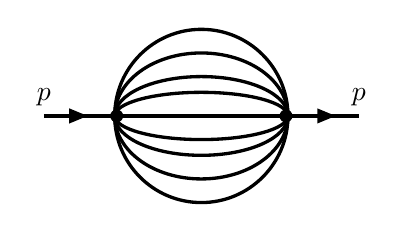
\begin{tikzpicture}[baseline=(x)]
        \begin{feynman}
       \vertex (x);
      \vertex[left=2cm of x,label=$p$](c1l);
      \vertex[right=2cm of x,label=$p$](c1r);
      \tikzfeynmanset{every vertex=dot}
        \vertex [left=1cm  of x] (xl);
        \vertex [right=1cm  of x] (xr);
        \draw [color = black, fill=none, very thick] (xl)  -- (xr);
        \draw [color = black, fill=none, very thick] (c1l)  -- (xl);
        \draw [color = black, fill=none, very thick] (xr)  -- (c1r);
        \diagram* {
         (c1l) -- [fermion] (xl);
         (xr) -- [fermion] (c1r);
         (xl)  [color = black, fill=none, very thick] -- (xr);
                                };
                              \end{feynman}
                                           \begin{pgfonlayer}{bg}
                                             \draw  [color = black, fill=none, very thick]  (x) circle (1.1cm);
                                              \draw  [color = black, fill=none, very thick] (x) ellipse (1.1cm
                                              and .8cm);
                                                \draw  [color = black, fill=none, very thick] (x) ellipse
                                                (1.1cm and .5cm);
                                                  \draw  [color =
                                                  black, fill=none,
                                                  very thick]  (x) ellipse (1.1cm and .3cm);
                        \end{pgfonlayer}
                   \end{tikzpicture}
  \caption{Multi-loop sunset}
  \label{fig:sunset}
\end{figure}

The $n-1$-loop sunset integral with $n\geq2$ in $D=2-2\epsilon$ dimensions reads
\begin{equation}
  I^{(n-1)}_\su(\vec m,t;\epsilon)= \int_{\Delta_n} \Omega^{(n-1)}_\su(\vec m,t,\epsilon)  ; \quad
  \Omega^{(n-1)}_\su(\vec m, t,\epsilon)={\Omega^{(n)}_0\over
    \textbf{F}_{n-1}(t)}\left(\textbf{U}_{n-1}^n\over \textbf{F}_{n-1}(t)^{n-1}\right)^\epsilon
\end{equation}
with
\begin{align}
  \textbf{ U}_{n-1}&= x_1\cdots x_n\sum_{i=1}^n {1\over x_i} \cr
      \textbf{   F}_{n-1}(t)&= \textbf{U}_{n-1} \sum_{i=1}^n m_i^2x_i-t x_1\cdots x_n
\end{align}
Notice that $\textbf{U}_{n-1}^n/ \textbf{F}_{n-1}(t)^{n-1}$ is an homogeneous
rational function  of degree
0 in $(x_1,\dots,x_n)$. As usual the differential form is defined in
the complement of the vanishing locus of the denominator in $\mathbb P^{n-1}\backslash\{\textbf{F}_{n-1}(t)=0\}$.
In $D=2$ dimension ($\epsilon=0$) we have a rational  differential form
$\Omega_\su(\vec m,t,0)$. The Picard-Fuchs operator has been
given up to six loop and is in agreement with the Feynman integral
being a (relative) period of a Calabi-Yau  manifold of complex dimension $n-2$~\cite{Bloch:2013tra,Bloch:2014qca,Bloch:2014qca,Bourjaily:2019hmc,Bonisch:2020qmm,Bonisch:2021yfw,Candelas:2021lkc,Forum:2022lpz}.

We apply the algorithm described in the previous section, with the
following results.
{\bf 


 We refer to the one-loop case in
   section~\ref{sec:one-loop-case}, the sunset two-loop case in
   section~\ref{sec:two-loop-case} for explicit examples in the smooth
   case. The non-smooth case of the all equal mass three-loop sunset
   is detailed in section~\pvnote{XXX}.
}
\begin{itemize}
  \item We rederive the differential operator for the one-loop bubble
    in Section~\ref{sec:one-loop-case}.
\item For the all equal mass case we will find that the $\epsilon$
deformation does not change the order of the minimal Picard-Fuchs
operator which is still $n-1$ at $n-1$ loop order. See
Section~\ref{sec:2sunset1mass} for the two-loop case, and at
higher-loop in Section~\ref{sec:highersunset1mass}. The results are
given on this page~\pvnote{sagenotebook}
\item The results for  generic mass two-loop sunset are given in
  Section~\ref{sec:2sunset3mass}
  \item The result for various mass configuration three-loop sunset
    are given in Section~\ref{sec:threeloop}
\end{itemize}


For the different masses cases the $\epsilon$ deformation does not
change the order of the differential operator at $l=1$- and $l=2$-loop
orders but changes the minimal order from  $l\geq3$ loops.
At one-loop order the differential operator is given by
\begin{multline}
    \mathscr{L}_\su^{(1)\epsilon} =
    \mathscr{L}_\su^{(0)1-mass}  + \epsilon 
    \left(\left(3 t^2-10
        t-9\right) {d\over dt}+(3t-5)\right)\cr +2 (t+1)
    \epsilon ^2
  \end{multline}
  and at two-loop order we have
  \begin{equation}
     \mathscr{L}^{(2)\epsilon}_\su =   \mathscr{L}^{a}_1
     \mathscr{L}^{b}_1    \mathscr{L}^{(2),0}_\su +\epsilon
     \mathscr{L}^{c}_4+\epsilon^2  \mathscr{L}^{d}_3+\epsilon^3
     \mathscr{L}^{e}_2+ \epsilon^4 \mathscr{L}^{f}_1 +\epsilon^5
   \mathscr{L}^{g}_0
   \end{equation} 
   where the operator $ \mathscr{L}^{x}_m$  with $x=a,b,c,d,e,g$ are
   of order $m$  and $ \mathscr{L}^{(2),0}_\su $ is the three
   different mass two-loop differential operator in $D=2$ derived in~\cite{Remiddi:2016gno,Bloch:2016izu,Muller-Stach:2011qkg}.
  

%------------------------------------------------------------------------
\subsection{Minimal differential equation for the one-loop sunset}\label{sec:one-loop-case}

We start with the one-loop case which illustrate the extension of the
Griffiths-Dwork reduction that will be applied to higher loop orders.


For the one-loop case the differential form is
\begin{equation}
  \Omega_\su^{(1)}(t)={1\over
    \textbf{F}_1(t)}\left(\textbf{U}_1^2\over \textbf{F}_1(t)\right)^\epsilon  \,\Omega_0^{(2)}
\end{equation}
with
\begin{align}
 \textbf{U}_1&=x_1+x_2\\
  \textbf{F}_1(t)&=-tx_1x_2+(x_1+x_2)(m_1^2x_1+m_2^2x_2).
\end{align}
We start with at the order $n=1$
\begin{equation}
{ d\over dt}
 \Omega^{(1)}_\su(t)= (1+\epsilon){x_1x_2\over (\textbf{F}_1(t))^2}
 \left(\textbf{U}_1^2\over \textbf{F}_1(t)\right)^\epsilon  \Omega_0^{(2)}
\end{equation}
%
We perform the Jacobian reduction of $x_1x_2$
\begin{equation}\label{e:reduc1loop}
 (1+\epsilon) x_1x_2= \sum_{i=1}^2 C_i^{(1)}\partial_i \textbf{F}_1(t)
\end{equation}
%
so that
\begin{equation}
{ d\over dt}
 \Omega^{(1)}_\su(t)= {\sum_{i=1}^2 C_i^{(1)}\partial^i \textbf{F}_1(t)\over (\textbf{F}_1(t))^2}
 \left(\textbf{U}_1^2\over \textbf{F}_1(t)\right)^\epsilon  \Omega_0^{(2)}
\end{equation}
this gives after integration by parts
\begin{multline}\label{e:PF1loopstep1}
 {d\over dt}
 \Omega^{(1)}_\su(t)=
 \left(-{\sum_{i=1}^2 \partial_i C_i^{(1)}\over
     (\textbf{F}_1(t))^2}-\epsilon{2\sum_{i=1}^2 C_i^{(1)}\partial_i
     \log \textbf{U}_1-\sum_{i=1}^2 C_i^{(1)}\partial_i
     \log \textbf{F}_1(t)\over \textbf{F}_1(t)}\right)\cr \times\left(\textbf{U}_1^2\over \textbf{F}_1(t)\right)^\epsilon \Omega_0+d\beta^{(1)}.
\end{multline}
%
with the boundary term defined by
\begin{equation}
  \beta^{(1)}=x_1  {C_1^{(1)}  \over  \textbf{F}_1(t) } \left(\textbf{U}_{1}^2\over
    \textbf{F}_1(t)\right)^\epsilon -  x_2  {C_2^{(2)}  \over  \textbf{F}_1(t) } \left(\textbf{U}_1^2\over
    \textbf{F}_1(t)\right)^\epsilon
\end{equation}
because $\beta^{(1)}= x_1 S_2-  x_2 S_1$ with $S_1$ and $S_2$ homogeneous
of degree $-1$ then $d\beta^{(1)}=- (\partial^1 S_1+\partial^2 S_2)
(x_2dx_1- x_1dx_2)$\footnote{This is an extension of the
  construction given by Griffith in~\cite{Griffiths_1969} This will be
  discussed again in details in section~\ref{sec:two-loop-case}.}, then we have 
\begin{equation}
  d\beta^{(1)}=- \sum_{i=1}^2 \partial^i  { C_i^{(1)}  \over
    \textbf{F}_1(t) } \left(\textbf{U}_1^2\over
    \textbf{F}_1(t)\right)^\epsilon\Omega_0^{(2)}.
\end{equation}
Using~\eqref{e:reduc1loop} one can rewrite~\eqref{e:PF1loopstep1} as
\begin{equation}
(1+\epsilon) {d\over dt}
 \Omega^{(1)}_\su(t)=
 \left({\sum_{i=1}^2 \partial_i C_i^{(1)}\over
     \textbf{F}_1(t)}+\epsilon{2\sum_{i=1}^2 C_i^{(1)}\partial_i
     \log \textbf{U}_1\over \textbf{F}_1(t)}\right)\left(\textbf{U}_1^2\over \textbf{F}_1(t)\right)^\epsilon \Omega_0+d\beta^{(1)}.
\end{equation}
We need to reduce the term $\sum_{i=1}^2 C_i^{(1)}\partial_i
     \log \textbf{U}_1$. For doing this we use the freedom from the
     syzygies
     \begin{equation}
       (\sigma_i)_{i=1,2}:=(x_1 \left(t-m_{1}^2-m_{2}^2\right)-2 m_{2}^2 x_2,x_2
       \left(m_{1}^2+m_{2}^2-t\right)+2 m_{1}^2 x_1)
     \end{equation}
     of the Jacobian ideal
   of $\textbf{F}_1$ such that $\sigma_1 \partial^1
   \textbf{F}_1+\sigma_2\partial^2 \textbf{F}_1=0$.
We seek a constant $\lambda$ such that
\begin{equation}\label{e:C1red}
  \sum_{i=1}^2 \left(C_i^{(1)}+ \lambda
      \sigma_i
  \right)  \partial_i \textbf{U}_1 = c^{(1)}\, \textbf{U}_1
\end{equation}
%
With this we can define 
\begin{align}
  \label{e:M1}
  M^{(1)}&:={\sum_{i=1}^2 \partial_i \left(C_i^{(1)}+\lambda
      \sigma_i
  \right) +2\epsilon
  c^{(1)}\over 1+\epsilon}\\
\nonumber &=\frac{\epsilon  \left(\left(m_{1}^2-m_{2}^2\right)^2-t^2\right)}{t
  (t-(m_1+m_2)^2)(t-(m_1-m_2)^2)}+\frac{m_{1}^2+m_{2}^2-t}{ (t-(m_1+m_2)^2)(t-(m_1-m_2)^2)}
\end{align}
the relation~\eqref{e:C1red} gives the reduction of pole
\begin{equation}
 {d\over dt}
 \Omega^{(1)}_\su(t)=
{M^{(1)}\over
    \textbf{F}_1(t)}\left(\textbf{U}_1^2\over \textbf{F}_1(t)\right)^\epsilon \Omega_0+d\beta^{(1)}.
\end{equation}
%
 which gives the differential equation $ \mathscr{L}_\su^{(1)}
 \Omega^{(1)}_\su(t) =d\beta^{(1)}$ with the Picard-Fuchs operator
 \begin{multline}\label{e:PF1loopresult}
\mathscr{L}_\su^{(1),\epsilon} =t
  (t-(m_1+m_2)^2)(t-(m_1-m_2)^2) {d\over dt}+t(t-m_{1}^2-m_{2}^2)\cr+\epsilon \left(t^2-\left(m_{1}^2-m_{2}^2\right)^2\right).
\end{multline}
The coefficient of order $\epsilon^0$ is the usual differential
operator for the one-loop sunset and we obtain the
$\epsilon$ dependence.
For the action of $ \mathscr{L}_\su^{(1)}$ on the one-loop Feynman
integral has an inhomogeneous term 
% 
\begin{equation}
  \mathscr{L}_\su^{(1)}  \int_{\Delta_1} \Omega_\su^{(1)}(t)=\int_{\Delta_1} d\beta^{(1)}
\end{equation}
We find for the inhomogeneous term
\begin{equation}
  \mathscr{S}_\su^{(1)}=- \left(m_{2}\over m_1\right)^{\epsilon }
   \left(-m_{1}^2+m_{2}^2+t\right)-\left(m_{1}\over m_2\right)^{\epsilon } 
   \left(m_{1}^2-m_{2}^2+t\right)  .
\end{equation}



%----------------------------------------------------------------------
\subsection{Differential equation for the  two-loop sunset}
\label{sec:two-loop-case}
We now turn to the two-loop sunset and shows how to adapt the
Griffiths-Dwork reduction used in~\cite{Bloch:2016izu,Lairez:2022zkj} to the $\epsilon$
dependent integrand.


For the two-loop case the differential form is
\begin{equation}\label{e:OmegaSunset}
  \Omega_\su^{(2)}(t)={1\over
    \textbf{F}_2(t)}\left(\textbf{U}_2^3\over \textbf{F}_2(t)^2\right)^\epsilon  \,\Omega_0^{(3)}
\end{equation}
with
\begin{align}
 \textbf{U}_2&=x_1x_2+x_1x_3+x_2x_3\\
  \textbf{F}_2(t)&=-tx_1x_2x_3 +U_3 (m_1^2x_1+m_2^2x_2+m_3^2x_3).
\end{align}
We first discuss the all equal mass term in
section~\ref{sec:2sunset1mass} and turn to the general mass case in section~\ref{sec:2sunset3mass}.


For the 

\pvnote{explain to order we start with using the bound from the euler
  characteristic}

\pvnote{The order is determined heuristically. First we have the upper
  bound from the previous result. Second we use special value since we
  only solve linear system to find the minimal order}
%----------------------------------------------------------------------
\subsection{The all equal mass case}\label{sec:2sunset1mass}
We derive the Picard-Fuchs equation satisfied by the two-loop all
equal mass in general dimensions. 
We  start with at the order $n=2$ 
\begin{equation}
 \left(d\over dt\right)^2
 \Omega_\su^{(2)}(t,\epsilon)={\Gamma(3+2\epsilon)\over\Gamma(1+2\epsilon)} {(x_1x_2x_3)^2\over \textbf{F}_2(t)^3}
 \left(\textbf{U}_2^3\over \textbf{F}_2(t)^2\right)^\epsilon  \Omega_0
\end{equation}
%
We perform the Jacobian reduction of $(x_1x_2x_3)^2$
\begin{equation}\label{e:reduc}
  {\Gamma(3+2\epsilon)\over\Gamma(1+2\epsilon)}\,  (x_1x_2x_3)^2= \sum_{i=1}^3 C_i^{(2)}\partial_i \textbf{F}_2(t)
\end{equation}
%
We introduce the differential form $\beta^{(2)}$ obtained by adapting the deriving in section~3.2
 of~\cite{Bloch:2016izu} to include the $\epsilon$ factor
 \begin{multline}
   \beta^{(2)}=   {x_2 \hat C_3^{(2)}-x_3 \hat C_2^{(2)}\over
   2  \textbf{F}_2(t)^2} \left(\textbf{U}_2^3\over \textbf{F}_2(t)^2\right)^\epsilon dx_1+   {x_3 \hat C_1^{(2)}-x_1 \hat C_3^{(2)}\over
    2 \textbf{F}_2(t)^2} \left(\textbf{U}_2^3\over \textbf{F}_2(t)^2\right)^\epsilon dx_2\cr
   +  {x_1 \hat C_2^{(2)}-x_2 \hat C_1^{(2)}\over
    2 \textbf{F}_2(t)^2} \left(\textbf{U}_2^3\over \textbf{F}_2(t)^2\right)^\epsilon dx_3.
 \end{multline}
which leads to using the same manipulations as in section~\ref{sec:non-rati-diff-form}
\begin{multline}
 (2+2\epsilon)\left(d\over dt\right)^2
 \Omega_\su(t,\epsilon)=
 \left({\sum_{i=1}^3 \partial_i C_i^{(2)}\over
     \textbf{F}_2(t)^{2}}+3\epsilon{\sum_{i=1}^3 C_i^{(2)}\partial_i
     \log \textbf{U}_2\over \textbf{F}_2(t)^{2}}\right)\cr \times\left(\textbf{U}_2^3\over \textbf{F}_2(t)^2\right)^\epsilon \Omega_0-d(2\beta^{(2)}).
\end{multline}
%
Performing the reduction for the shifted coefficients by the syzygies
of the Jacobian of $\textbf{F}_2(t)$
\begin{equation}
    \hat C_i^{(2)}:=C_i^{(2)}+\sum_{k=1}^4 \lambda_k
      \sigma^k_i \qquad \textrm{for}\qquad i=1,2,3
    \end{equation}
    where $\lambda_k$ are unknown homogeneous degree 4 polynomials in
$(x,y,z)$ .
We have to solve the following equation for $\lambda_k$  and $c^{(2)}$ is an unknown homogeneous degree 3 polynomial
in $(x,y,z)$
\begin{equation}\label{e:C2red}
  \sum_{i=1}^3 \hat C_i^{(2)} \partial^i \textbf{U}_2 = c^{(2)} \textbf{U}_2
\end{equation}
The unknown are fully determined at the end of  algorithm.
Defining 
\begin{equation}
  \label{e:M2}
  M^{(2)}:={\sum_{i=1}^3 \partial^i \hat C_i^{(2)}+3\epsilon
    c^{(2)}\over 2+2\epsilon}
\end{equation}
the relation~\eqref{e:C2red} gives the reduction of pole
\begin{equation}
 \left(d\over dt\right)^2
 \Omega_\su(t,\epsilon)=
{M^{(2)}\over
     \textbf{F}_2^{2}}\left(\textbf{U}_2^3\over \textbf{F}_2(t)^2\right)^\epsilon \Omega_0+d\beta^{(2)},
 \end{equation}
%
We now add the first derivative with an unknown rational coefficient $c_1(t,\epsilon)$
\begin{multline}
 \left(d\over dt\right)^2
 \Omega_\su(t,\epsilon) +c_1(t,\epsilon) \left(d\over dt\right)
 \Omega_\su(t,\epsilon) \cr=
{M^{(2)}+c_1(t,\epsilon) x_1x_2x_3(1+2\epsilon)\over
     \textbf{F}_2(t)^{2}}\left(\textbf{U}_2^3\over \textbf{F}_2(t)^2\right)^\epsilon \Omega_0+d\beta^{(2)}
 \end{multline}
 We then reduce the pole by writing
 \begin{equation}\label{e:M2red}
   M^{(2)}+ c_1(t,\epsilon) x_1x_2x_3(1+2\epsilon)= \sum_{i=1}^3
   C_i^{(1)} \partial^i \textbf{F}_2(t)
 \end{equation}
leading to
\begin{equation}
 \left(d\over dt\right)^2
 \Omega_\su(t,\epsilon) +c_1(t,\epsilon) \left(d\over dt\right)
 \Omega_\su(t,\epsilon) =
{ \sum_{i=1}^3
   C_i^{(1)} \partial^i \textbf{F}_2(t)\over
     \textbf{F}_2(t)^{2}}\left(\textbf{U}_2^3\over \textbf{F}_2(t)^2\right)^\epsilon \Omega_0+d\beta^{(2)}
 \end{equation}
 where $ C_i^{(1)}$ are unknown homogeneous degree 1 polynomials in $(x,y,z$).
We now impose the 
\begin{equation}\label{e:c0}
  \sum_{i=1}^3C_i^{(1)}\partial^i \textbf{F}_2(t)+ c_0(t,\epsilon) \textbf{F}_2 (t) =0.
\end{equation}
%
The equations~\eqref{e:C2red},~\eqref{e:M2red} and~\eqref{e:c0} lead
to the unique solution for the coefficients $c_1$ and $c_0$.
We have the solutions
\begin{align}
  c_1(t,\epsilon)&=\frac{\left(3 t^2-10 t-9\right) \epsilon }{(t-9) (t-1) t}+\frac{3 t^2-20 t+9}{(t-9) (t-1)
   t}\cr
  c_0(t,\epsilon)&=\frac{\epsilon ^2 (2 t+2)}{(t-9) (t-1) t}+\frac{\epsilon  (3 t-5)}{(t-9) (t-1)
   t}+\frac{t-3}{(t-9) (t-1) t}  .
\end{align}
leading to the $\epsilon$-deformed Picard-Fuchs operator
\begin{multline}
  \label{e:PF2sunset1massepsilon}
     \mathscr{L}^{(2),\epsilon,1-mass}_\su ={d\over dt}\left( t(t-1)(t-9)
       {d\over dt}\right)+(t-3)\cr+\epsilon\left((3t^2-10t-9) {d\over
         dt}+3t-5\right)
     +\epsilon^2 2(t+1).
\end{multline}
%



The inhomogeneous term is given by evaluating the integral 
\begin{equation}
  S_\epsilon^{(2)}=\int_{\Delta_2} d\beta^{(2)} .
\end{equation}
The inhomogeneous term is defined as usual in the Griffiths-Dwork
reduction as (see section~3.2 of~\cite{Bloch:2016izu})
\begin{multline}
  \beta^{(2)}= {x_2 C_3^{(2)} -x_3 C_2^{(2)}\over \textbf{F}_2(t)}
  \left(\textbf{U}_2^3\over \textbf{F}_2(t)^2\right)^\epsilon  dx_1
  + {x_3 C_1^{(2)} -x_1 C_3^{(2)}\over \textbf{F}_2(t)}
  \left(\textbf{U}_2^3\over \textbf{F}_2(t)^2\right)^\epsilon  dx_2\cr+ {x_1 C_2^{(2)} -x_2 C_1^{(2)}\over \textbf{F}_2(t)}
  \left(\textbf{U}_2^3\over \textbf{F}_2(t)^2\right)^\epsilon  dx_3
\end{multline}
this time including the $\epsilon$ dependent factor. 
Because the denominator of $\beta^{(2)}$ has a pole at the coordinate
point $[1:0:0]$, $[0:1:0]$ and $[0:0:1]$ one needs to consider the
blow-up  of the domain of integration $\Delta_2$ by inserting a small
$\mathbb P^1$ of radius $\varepsilon$ (see eq.~(3.47) of~\cite{Bloch:2016izu})
\begin{equation}
    S_\epsilon^{(2)}=\lim_{\epsilon\to0} \sum_{i=1}^3
    \int_{\partial\tilde\Delta_2|_{x_i=0}} \sum_{1\leq j\neq i\leq 3}
    \beta_j dx_j
\end{equation}
A computation identical to the one performed in~\cite{Bloch:2016izu} leads to
the result
\begin{equation}
  S_\epsilon^{(2)}=  -6 \, {\Gamma(1+\epsilon)^2\over \Gamma(1+2\epsilon)}
\end{equation}
The piece of order $\epsilon^0$ reproduces the Picard-Fuchs operator
for the two-loop all equal-mass sunset in $D=2$ given
in~\cite{Bloch:2013tra,Bloch:2013tra,Vanhove:2014wqa,Bonisch:2020qmm,Pogel:2022vat}.

%----------------------------------------------------------------------
\subsection{The different mass case}\label{sec:2sunset3mass}

For the non equal mass case the order of the differential equation is
4 with the following $\epsilon$ expansion
\begin{equation}
     \mathscr{L}^{(2),\epsilon}_\su =   \mathscr{L}^{(1)}_1
     \mathscr{L}^{(2)}_1    \mathscr{L}^{3-mass}_\su +\epsilon
     \mathscr{L}^{(3)}_4+\epsilon^2  \mathscr{L}^{(4)}_3+\epsilon^3
     \mathscr{L}^{(5)}_2+ \epsilon^4 \mathscr{L}^{(6)}_1 +\epsilon^5
    \mathscr{L}^{(7)}_0
   \end{equation} 
   where $ \mathscr{L}^{(r)}_m$  are irreducible differential operator
   of  order $m$ and $\mathscr{L}^{3-mass}_\su$ is the differential
   operator for the three-mass two-loop sunset integral in two
   dimensions. This differential equation reproduces the one 
   derived~\cite{Remiddi:2013joa,Remiddi:2016gno}.

The $\epsilon$ deformation does not change the non-apparent
singularities of the differential operator as can be seen from the
coefficient of the highest order term
\begin{multline}
  \mathscr{L}^{(2),\epsilon}_\su \Big\vert_{(d/dt)^4}= t^3\prod_{i=1}^4 (t-
  \mu_i^2) \Big(-\left(2 \epsilon +5\right) t^{2}-2
    \left(m_{1}^{2}+m_{2}^{2}+m_{3}^{2}\right) \left(1+2 \epsilon
    \right) t \cr+ \left(7+6 \epsilon \right)\prod_{i=1}^4 \mu_i
\Big)  
\end{multline}
where $\mu_i=\{m_1+m_2+m_3,-m_1+m_2+m_3,m_1-m_2+m_3,m_1+m_2-m_3\}$ are
the thresholds.  The $\epsilon$ deformation is only affecting the
apparent singularities, since the $\epsilon$ factor
in~\eqref{e:OmegaSunset} does not change the nature of the singular
locus which is still given by the same elliptic curve as in the
$\epsilon=0$ case.
   
Its actions on the Feynman integral is given by 
\begin{equation}
     \mathscr{L}^{(2),\epsilon}_\su  I(\underline
     m,t;\epsilon)=\mathscr{S}(\vec m,t;\epsilon) 
   \end{equation}
   with the source term
   \begin{equation}
     \mathscr{S}(\vec m,t;\epsilon)=\frac{c_{23}(t,\epsilon)\Gamma (\epsilon +1)^2}{ (m_{2} m_{3})^{2 \epsilon}\Gamma (1+2\epsilon)}+\frac{c_{13}(t,\epsilon)\Gamma (\epsilon +1)^2}{ (m_{1} m_{3})^{2 \epsilon }\Gamma (1+2
   \epsilon)}+\frac{c_{12}(t,\epsilon)\Gamma (\epsilon +1)^2}{ (m_{1} m_{2})^{2 \epsilon }\Gamma (1+2
   \epsilon )}
\end{equation}
where $c_{12}(t,\epsilon)$, $c_{13}(t,\epsilon)$ and
$c_{23}(t,\epsilon)$ are polynomials of degree 4 in $t$ and 2 in
$\epsilon$. \pvnote{given on page}

This has the small $\epsilon$ series expansion
\begin{equation}
    \mathscr{S}(\vec m,t;\epsilon)=\mathscr{S}^0(\vec m,t)
    +\left(c^{(1)}_0(\vec m)+
    \sum_{i=1}^3  c^{(1)}_i(\vec m)\log(m_i)\right)\,  \epsilon+O(\epsilon^2)
\end{equation}
with  the leading term given by
   \begin{equation}
   \mathscr{S}^0(\vec m,t)=60 t^{4}+56\left( m_{1}^{2}+ m_{2}^{2}+
     m_{3}^{2}\right) t^{3}
   -308 \prod_{i=1}^4 \mu_i.
 \end{equation}
For $\epsilon=0$ the two-loop sunset integral satisfies  the
differential equation
\begin{equation}
  \mathscr{L}^{3-mass}_\su f_\su^{(0)}(t)= s_0(\vec m,t)+ \sum_{i=1}^3
  s_i(\vec m,t)\log(m_i^2)  
\end{equation}
with \pvnote{given on the page}
\begin{align}
  s_0(\vec m,t)&:=18 t^{4}-24\left(m_{1}^{2}m_{2}^{2}+
       m_{3}^{2}\right) t^{3}-4\left( m_{1}^{4}+m_2^4+m_3^4+10(
       m_{1}^{2} m_{2}^{2}+ m_{1}^{2}
       m_{3}^{2}+m_{2}^{2}
       m_{3}^{2})\right) t^{2}\cr
       &+8
       \left(m_{1}^{2}+m_{2}^{2}+m_{3}^{2}\right)\prod_{i=1}^4\mu_i
       t +2 \prod_{i=1}^4\mu_i^2 \cr
  s_1(\vec m,t)&=\left(4 m_{1}^{2}-2 m_{2}^{2}-2 m_{3}^{2}\right)
       t^{3}+\left(-12 m_{1}^{4}+14 m_{1}^{2} m_{2}^{2}+14 m_{1}^{2}
       m_{3}^{2}+6 m_{2}^{4}-28 m_{2}^{2} m_{3}^{2}+6 m_{3}^{4}\right)
       t^{2}\cr
       &+\Big(12 m_{1}^{6}-22 m_{1}^{4} m_{2}^{2}-22 m_{1}^{4} m_{3}^{2}+16 m_{1}^{2} m_{2}^{4}+16 m_{1}^{2} m_{3}^{4}-6 m_{2}^{6}+6 m_{2}^{4} m_{3}^{2}+6 m_{2}^{2} m_{3}^{4}\cr&-6 m_{3}^{6}\Big) t-2 \left(2 m_{1}^{4}-m_{1}^{2} m_{2}^{2}-m_{1}^{2} m_{3}^{2}-m_{2}^{4}+2 m_{2}^{2} m_{3}^{2}-m_{3}^{4}\right) \prod_{i=1}^4\mu_i\cr
       s_2(\vec m,t)&=\left(-2 m_{1}^{2}+4 m_{2}^{2}-2 m_{3}^{2}\right)
            t^{3}+\left(6 m_{1}^{4}+14 m_{1}^{2} m_{2}^{2}-28
            m_{1}^{2} m_{3}^{2}-12 m_{2}^{4}+14 m_{2}^{2} m_{3}^{2}+6
            m_{3}^{4}\right) t^{2}\cr
            &+\Big(-6 m_{1}^{6}+16 m_{1}^{4} m_{2}^{2}+6 m_{1}^{4} m_{3}^{2}-22 m_{1}^{2} m_{2}^{4}+6 m_{1}^{2} m_{3}^{4}+12 m_{2}^{6}-22 m_{2}^{4} m_{3}^{2}+16 m_{2}^{2} m_{3}^{4}\cr&-6 m_{3}^{6}\Big) t +2 \left(m_{1}^{4}+m_{1}^{2} m_{2}^{2}-2 m_{1}^{2} m_{3}^{2}-2 m_{2}^{4}+m_{2}^{2} m_{3}^{2}+m_{3}^{4}\right) \prod_{i=1}^4\mu_i
\cr
            s_3(\vec m,t)&=-s_1-s_2.
\end{align}
It can be checked that 
\begin{equation}
  \mathscr{S}^0(\vec m,t)=   \mathscr{L}^{(1)}_1
     \mathscr{L}^{(2)}_1    \mathscr{L}^{3-mass}_\su  f_\su^{(0)}(t).
\end{equation}
The logarithmic dependence on the masses arise at the order $\epsilon$ 
 and
 \begin{align}
&     c^{(1)}_0(\vec m)=114 t^{4}+168\left(m_{1}^{2}+ m_{2}^{2}+ m_{3}^{2}\right)
  t^{3}+\Big(-552 (m_{1}^{4}+m_2^4+m_3^4)\cr&+1136 (m_{1}^{2} m_{2}^{2}+
    m_{1}^{2} m_{3}^{2}+ m_{2}^{2} m_{3}^{2})\Big) t^{2}-64
  \left(m_{1}^{2}+m_{2}^{2}+m_{3}^{2}\right) \prod_{i=1}^4\mu_i t +14 \prod_{i=1}^4\mu_i^2\\
& c^{(1)}_1(m_1,m_2,m_3)=-80 t^{4}-\left( 88 m_{1}^{2}+ 68 m_{2}^{2}+68 m_{3}^{2}\right)
 t^{3}+\Big(360 m_{1}^{4}-780 m_{1}^{2} m_{2}^{2}-780 m_{1}^{2}
   m_{3}^{2}\cr&+436 m_{2}^{4}-904 m_{2}^{2} m_{3}^{2}+436
   m_{3}^{4}\Big) t^{2}+\Big(-136 m_{1}^{6}+324 m_{1}^{4}
   m_{2}^{2}+324 m_{1}^{4} m_{3}^{2}-256 m_{1}^{2} m_{2}^{4}\cr&-256
   m_{1}^{2} m_{3}^{4}+68 m_{2}^{6}-68 m_{2}^{4} m_{3}^{2}-68
   m_{2}^{2} m_{3}^{4}+68 m_{3}^{6}\Big) t -28   \prod_{i=1}^4\mu_i\cr&\times\Big(2 m_{1}^{4}-m_{1}^{2} m_{2}^{2}-m_{1}^{2} m_{3}^{2}-m_{2}^{4}+2 m_{2}^{2} m_{3}^{2}-m_{3}^{4}\Big) 
\end{align}
with $c^{(1)}_2(m_1,m_2,m_3)=c^{(1)}_1(m_2,m_1,m_3)$ and $c^{(1)}_3(m_1,m_2,m_3)=c^{(1)}_1(m_3,m_2,m_1)$.
and $c^{(1)}_1(\vec m)+c_2^{(1)}(\vec m)+c_3^{(1)}(\vec m)=4
\mathscr{S}^0(\vec m,t)$.


%----------------------------------------------------------------------
\subsection{Minimal differential operator for higher-loop sunset}

We now turn to the higher loop case. We first discuss the all equal
mass case and then a numerical example at three-loop order with all
possible mass configurations.
%----------------------------------------------------------------------   
   \subsubsection{The all equal mass case}\label{sec:highersunset1mass}
Already in $D=2$ dimensions, for the sunset integral from three loop
and higher  the Griffiths-Dwork algorithm had to be adapted because of
the non-isolated singularities of integrand. This was achieved
in~\cite{Lairez:2022zkj} by using syzygies. The resolution of the
linear system in eq.~\eqref{e:sysCFU} takes into account the syzygies
when including the $\epsilon$ dependent factor.   The computation
takes a rather long time
since this involves solving large linear systems. \pvnote{finiteflow}

   
For the all equal mass case $m_1=\cdots =m_{l+1}=1$ we find the sunset
Feynman integral satisfies the differential equation
\begin{equation}
  \mathscr{L}_\su^{(l),\epsilon} I_\su(\{1,\dots,1\},t,\epsilon)=
  -(l+1)! {\Gamma(1+\epsilon)^l\over \Gamma(1+l\epsilon)}
\end{equation}
with
\begin{equation}
  \mathscr{L}_\su^{(l),\epsilon} =\sum_{r=0}^{l}  \mathscr{L}_\su^{(l),r} \epsilon^r
\end{equation}
where the differential operator is $ \mathscr{L}_\su^{(l),r}$ is of
order $l-r$. The Picard-Fuchs operator $ \mathscr{L}_\su^{(l),0}$ is
the one derived in~\cite{Vanhove:2014wqa} up to five-loops (see as well~\cite{Bonisch:2020qmm,Pogel:2022yat,Pogel:2022ken,Pogel:2022vat}).

The results for the differential equation are given on this
page~\pvnote{give sagenotebook}
%-------------------------------------------------------------------------
\subsubsection{The three-loop generic mass cases}\label{sec:threeloop}

For the three-loop sunset with different masses we find the following
results. We follow the notation of section~4 of~\cite{Lairez:2022zkj}

\begin{itemize}
\item  {\bf Case~$[4]$:} The all equal mass case $m_1=m_2=m_3=m_4$ has already been
  discussed in the previous section. The Picard-Fuchs operator is of order 3 is given by
  \begin{multline}
    \mathscr{L}_\su^{[4],\epsilon}=
    -(t - 16)  (t - 4)  t^2\left(d\over dt\right)^3 - 6  (t^3 -
                              15  t^2 + 32  t)  \left(d\over dt\right)^2 - (7  t^2 - 68  t +
                              64)  \left(d\over dt\right) - t + 4\cr
                              +\epsilon \left(-6  (t - 10  ) t^2 \left(d\over dt\right)^2 -
      6  (3  t - 20  ) t \left(d\over dt\right) +18- 6  t 
      \right)\cr
    +\epsilon^2\left(-(11  t^2 -
      28  t - 64)  \left(d\over dt\right) - 11  t + 14\right)+ \epsilon^3\left(-6  t - 12\right)
  \end{multline}
the $\epsilon^0$ operator is the operator derived and analysed in~\cite{Vanhove:2014wqa,Bloch:2014qca,Pogel:2022yat}


  \item   {\bf Case~$[31]$:} For two different masses $m_1=m_2=m_3 \neq m_4$ the
  Picard-Fuchs operator is of order 5 and has the $\epsilon$ dependence
  \begin{equation}
    \mathscr{L}^{[31],\epsilon}_\su=       \sum_{r=0}^1 \epsilon^r
    \mathscr{L}^{[31],r}_{5}+  \sum_{r=0}^4 \epsilon^{2+r}   \mathscr{L}^{[31],r}_{4-r}
  \end{equation}
  where  $ \mathscr{L}^{[31],r}_{n}$ are of order $n$.
  The order $\epsilon^0$ operator factorizes as
  \begin{equation}
         \mathscr{L}^{[31],0}_{5}=   \mathscr{L}^{[31],0}_{a,1} \mathscr{L}^{[31],\epsilon}_\su
       \end{equation}
        where  $ \mathscr{L}^{[31],0}_{a,1}$ is a  first order operator
       and $\mathscr{L}^{[31],0}_\su$ is the fourth order
       Picard-Fuchs operator the
       three-loop sunset integral with mass configuration $[31]$ given
       in section~4.3 of~\cite{Lairez:2022zkj}.
       The coefficient of the highest order term $(d/dt)^5$    is given by
       \begin{multline}
                   \mathscr{L}^{[31],\epsilon}_\su\Big\vert_{(d/dt)^5}=
                   t^3  (t-(m_1-m_4)^2)(t-(m_1+m_4)^2)(t-(3m_1+m_4)^2) \cr\times (t-(3m_1-m_4)^2)
            q^{[31]}(t,\epsilon)      .
                 \end{multline}
                 The $\epsilon$ dependence appears only in the
                 apparent singularities determined by the polynomial
                 $q^{[31]}(t,\epsilon)$ of degree 3 in $t$ and 1 in $\epsilon$.
\item   {\bf Case~$[22]$:} For two different masses $m_1=m_2\neq m_3 = m_4$ the
  Picard-Fuchs operator has order 6 and the $\epsilon$ expansion 
  \begin{equation}
    \mathscr{L}^{[22],\epsilon}=     \sum_{r=0}^3 \epsilon^r
    \mathscr{L}^{[22],r}_{6}+  \sum_{r=0}^5 \epsilon^{4+r}   \mathscr{L}^{[22],r}_{5-r}
  \end{equation}
  where  $ \mathscr{L}^{[22],r}_{n}$ are 
  operators of order $n$.
  The order $\epsilon^0$ operator factorizes as
  \begin{equation}
         \mathscr{L}^{[22],0}_{6}=   \mathscr{L}^{[22],0}_{a,1} \mathscr{L}^{[22],0}_{b,1}\mathscr{L}^{[22],0}_\su
       \end{equation}
       where  $ \mathscr{L}^{[22],0}_{a,1}$ and $
       \mathscr{L}^{[22],0}_{b,1}$ are first order operators
       and $\mathscr{L}^{[22],0}_\su$ is the fourth order operator for the
       three-loop sunset integral with mass configuration $[22]$ given  section~4.3 of~\cite{Lairez:2022zkj}.
    The coefficient of the highest order term $(d/dt)^6$    is given by
       \begin{multline}
                   \mathscr{L}^{[22],\epsilon}_\su\Big\vert_{(d/dt)^6}=
                   t^4(t-(2m_1)^2)(t-(2m_4)^2)(t-(2m_1+2m_4)^2)\cr\times(t-(2m_1-2m_4)^2)
                   \, q^{[22]}(t,\epsilon).
                 \end{multline}
                 The $\epsilon$ dependence appears only in the
                 apparent singularities determined by the polynomial
                 $q^{[22]}(t,\epsilon)$ of degree 4 in $t$ and $3$ in $\epsilon$.
     \item   {\bf Case~$[211]$:}For three different masses $m_1=m_2\neq m_3 \neq m_4$ the
  Picard-Fuchs operator has order 7 and has the $\epsilon$ expansion
  \begin{equation}
    \mathscr{L}^{[211],\epsilon}_\su=       \sum_{r=0}^8 \epsilon^r
    \mathscr{L}^{[211],r}_{7}+  \sum_{r=0}^6 \epsilon^{9+r}   \mathscr{L}^{[22],r}_{6-r}
  \end{equation}
   where  $ \mathscr{L}^{[211],r}_{n}$ 
  are operators of order $n$.
    The order $\epsilon^0$ operator factorizes as
  \begin{equation}
         \mathscr{L}^{[211],0}_{7}=   \mathscr{L}^{[211],0}_{a,1}  \mathscr{L}^{[211],0}_{b,1} \mathscr{L}^{[211],0}_{c,1}\mathscr{L}^{[211],0}_\su
       \end{equation}
        where  $ \mathscr{L}^{[211],0}_{a,1}$,  $
        \mathscr{L}^{[211],0}_{b,1}$ and  $ \mathscr{L}^{[211],0}_{c,1}$ are  first order operators
       and $\mathscr{L}^{[211],0}_\su$ is the fifth order Picard-Fuchs operator the
       three-loop sunset integral with mass configuration $[211]$
       given section~4.3 of~\cite{Lairez:2022zkj}.   The coefficient of the highest order term $(d/dt)^6$    is given by
       \begin{multline}
                   \mathscr{L}^{[211],\epsilon}_\su\Big\vert_{(d/dt)^6}=
                   t^5\left(t-(m_{1}-m_{2})^2\right) \left(t-(m_{1}+m_{2})^2\right)\cr\times
   \left(t-(m_{1}+m_{2}-2 m_{4})^2\right) \left(t-(m_{1}-m_{2}+2
   m_{4})^2\right) \left(t-(-m_{1}+m_{2}+2 m_{4})^2\right)\cr\times
   \left(t-(m_{1}+m_{2}+2 m_{4})^2\right)
                   \, q^{[211]}(t,\epsilon).
                 \end{multline}
                 The $\epsilon$ dependence appears only in the
                 apparent singularities determined by the polynomial
                 $q^{[211]}(t,\epsilon)$ of degree 9 in $t$  and 7 in $\epsilon$.
  \item   {\bf Case~$[1111]$:} For four different masses $m_1\neq m_2\neq m_3 \neq m_4$ the
  Picard-Fuchs operator has order 11 and has the $\epsilon$ expansion 
  \begin{equation}
    \mathscr{L}^{[1111],\epsilon}=     \sum_{r=0}^{16}\epsilon^r
    \mathscr{L}^{[1111],r}_{11}+\sum_{r=0}^{11} \epsilon^{16+r}  \mathscr{L}^{[1111],\epsilon}_{11-r}
  \end{equation}
    The order $\epsilon^0$ operator factorizes as
  \begin{equation}
         \mathscr{L}^{[1111],0}_{0,11}=   \mathscr{L}^{[1111],0}_{a_1,1}  \cdots  \mathscr{L}^{[1111],0}_{a_5,1}   \mathscr{L}^{[1111],0}_{\su}
       \end{equation}
        where  $ \mathscr{L}^{[1111],\epsilon}_{a_1,1},\dots,  \mathscr{L}^{[1111],\epsilon}_{a_5,1}$ are  first order operators
       and $\mathscr{L}^{[1111],0}_{\su}$ is the sixth  order  Picard-Fuchs operator for the
       three-loop sunset integral with mass configuration $[1111]$
       given in~\cite{Lairez:2022zkj}.
        The coefficient of the highest order term $(d/dt)^{11}$    is given by
       \begin{multline}
                   \mathscr{L}^{[1111],\epsilon}_\su\Big\vert_{(d/dt)^{11}}=
                   t^{11}\left(t-(m_{1}+m_{2}-m_{3}-m_{4})^2\right) \cr\times
   \left(t-(m_{1}-m_{2}+m_{3}-m_{4})^2\right)
   \left(t-(m_{1}+m_{2}+m_{3}-m_{4})^2\right) \cr\times
   \left(t-(m_{1}-m_{2}-m_{3}+m_{4})^2\right)
   \left(t-(m_{1}+m_{2}-m_{3}+m_{4})^2\right)\cr\times
   \left(t-(m_{1}-m_{2}+m_{3}+m_{4})^2\right)
   \left(t-(-m_{1}+m_{2}+m_{3}+m_{4})^2\right) \cr\times
   \left(t-(m_{1}+m_{2}+m_{3}+m_{4})^2\right)
                   \, q^{[1111]}(t,\epsilon).
                 \end{multline}
                 The $\epsilon$ dependence appears only in the
                 apparent singularities determined by the polynomial
                 $q^{[1111]}(t,\epsilon)$ of degree 17 in
                 $t$ and 16 in $\epsilon$.
     \end{itemize}
\pvnote{correlation between the order in epsilon and the degree of
  apparent singularities}
%--------------------------------------------------------------------
\subsubsection{The Bessel representation}


Following the steps in section~8 of~\cite{Vanhove:2014wqa}
gives the following Bessel integral representation for the multiloop
sunset integral in  $D=2-2\epsilon$ dimensions
\begin{multline}
  I^{(n-1)}(\vec m,t;\epsilon)=
  {2^{(n-1) (1-\epsilon)} t^{\epsilon\over2} \over    (m_1\cdots m_{L+1})^{\epsilon}
  \Gamma(1+(n-1)\epsilon)}\cr\times\int_0^\infty I_{-\epsilon}(\sqrt{t} x)
  \prod_{i=1}^{L+1}K_{-\epsilon}(m_ix)\,  x^{1+\epsilon(n-1)}dx.
\end{multline}
This integral representation is valid for   for $t<(m_1+\cdots +m_{n})^2$.
%
For $x\to0$ we have
\begin{equation}
  \lim_{x\to0} I_{-\epsilon}(x)\simeq \left(x\over2\right)^{\epsilon};    \qquad
  \lim_{x\to0} K_{-\epsilon}(x)   \simeq \left(x\over2\right)^{\epsilon}
\end{equation}
and the integral converges as long as $2+(n-1)\epsilon>0$ which is the
condition $D=2-2\epsilon< 2n/(n-1)$ for the absence of UV divergences
for the $n-1$-loop massive sunset.

Using this representation and applying the creative telescoping
algorithm~\cite{Chyzak,Chyzak2,bostan2013creative,Koutchan} we have checked the results obtained the
extended Griffiths-Dwork reduction.
The creative telescoping algorithm builds an annihilator
\begin{equation}
  \mathscr{T}(t,\partial_t; x,\partial_x)= \mathscr{L}(t,\partial_t)+ \mathscr{C}(  t,\partial_t; x,\partial_x)
\end{equation}
of the integrand
$i(t,x):= I_{-\epsilon}(\sqrt{t} x)
  \prod_{i=1}^{L+1}K_{-\epsilon}(m_ix)\,  x^{1+\epsilon(n-1)}$
such that
\begin{equation}
      \mathscr{T}(t,\partial_t; x,\partial_x) i(t,x)=\mathscr{L}(t,\partial_t)i(t,x)+ \mathscr{C}(  t,\partial_t; x,\partial_x) i(t,x)=0
    \end{equation}
    implying that $\mathscr{L}(t,\partial_t)i$ is the operator acting
    on the integral because the domain of integration is independent
    of $t$.
For the multi-loop sunset
integrals this is the fastest way of obtaining these results as it
only takes only from a few second to a few minutes for deriving the
results to high-loop order for the all equal mass case. Notice as well
that the algorithm gives the minimal  differential operator and does
not need any factorisation step to the contrary to the algorithm
presented in~\cite{Pogel:2022vat}. The irreducibility is not guaranteed
but it can be checked easily with the algorithm~\cite{chyzak2022symbolic,goyer2021sage}. It
turns that for the sunset integrals the algorithms produces the
minimal order differential operator.

     
%%%%%%%%%%%%%%%%%%%%%%%%%%%%%%%%%%%%%%%%%%%%%%%%%%%%%%%%%%%%%%%%%%
\section{The ice-cream cone in general dimensions}\label{sec:ice-cream}

\begin{figure}[h]
  \centering
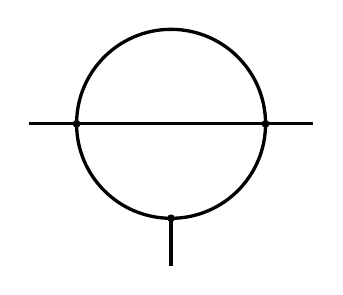
\begin{tikzpicture}[scale=0.6]
\filldraw [color = black, fill=none, very thick] (0,0) circle (2cm);
\draw [black,very thick] (-2,0) to (2,0);
\filldraw [black] (2,0) circle (2pt);
\filldraw [black] (0,-2) circle (2pt);
\filldraw [black] (-2,0) circle (2pt);
\draw [black,very thick] (-2,0) to (-3,0);
\draw [black,very thick] (2,0) to (3,0);
\draw [black,very thick] (0,-2) to (0,-3);
\end{tikzpicture}
\caption{The ice cream cone graph}\label{fig:icecream}
\end{figure}

In this Section we give the result for the $\epsilon$-deformed
differential equation for the ice-cream cone graph generalising the result
for $\epsilon=0$ given in~\cite{Lairez:2022zkj,Doran:2023yzu}.

The two-loop (one scoop) ice-cream cone  differential form in
$D=2-2\epsilon$ dimensions is given by
\begin{equation}
  \omega_{(2,1,1),  2-2\epsilon}(t)= {\textbf{U}_{(2,1,1)}\over
    (\textbf{F}_{(2,1,1);2-2\epsilon})^2} \left(\textbf{U}_{(2,1,1)}^3\over  (\textbf{F}_{(2,1,1);2-2\epsilon})^2\right)^{\epsilon}
\end{equation}

with
\begin{align}
  \textbf{U}_{(2,1,1)}&:=(y_1+y_2)(x_1+z)+zx_1,\cr
                        \textbf{V}_{(2,1,1)}&:=p_2^2y_1y_2(z+x_1)+zx_1(p_1^2y_1+p_2^2y_2),\\
\nonumber  \textbf{F}_{(2,1,1);D}(t)&:=\textbf{U}_{(2,1,1)}
                             (\mu_1^2y_1+\mu_2^2y_2^2+m_1^2x_1+m_2^2z)-t \textbf{V}_{(2,1,1);D}.
\end{align}

We find the following results (some numerical cases are accessible on
the page \pvnote{PF-Ice-cream-epsilon.ipynb})
\begin{itemize}
\item {\bf The all equal kinematics
  $\mu_1=\mu_2=m_1=m_2=p_1^2=p_2^2=p_3^2=1$:} the Picard-Fuchs operator
  has order 3 and
  reads
  \begin{equation}
        \mathscr{L}_{(2,1,1)}^{[7],\epsilon}=\sum_{r=0}^4 \epsilon^r\,\mathscr{L}_{(2,1,1)}^{[7],r}
      \end{equation}
with
  \begin{align}
\mathscr{L}_{(2,1,1)}^{[7],0}&= 2 t^{3} \left(t -1\right)
\left(t -3\right) \left(t -4\right) \left(d\over dt\right)^{3}+2 t^{2} \left(t
  -2\right) \left(11 t^{2}-44 t +15\right) \left(d\over dt\right)^{2}\cr&+2 t^{2}
\left(29 t^{2}-116 t +89\right) {d\over dt} +32 t^{2} \left(t
  -2\right)\cr
\mathscr{L}_{(2,1,1)}^{[7],1}&=t^{3} \left(t -1\right) \left(t -3\right) \left(t -4\right) \left(t +1\right) \left(d\over dt\right)^{3}+t^{2} \left(10 t^{4}-37 t^{3}-26 t^{2}+95 t +18\right) \left(d\over dt\right)^{2}\cr&+t \left(24 t^{4}+5 t^{3}-242 t^{2}+53 t +48\right)  {d\over dt} +12 t^{4}+64 t^{3}-112 t^{2}-48 t -12,\cr
\mathscr{L}_{(2,1,1)}^{[7],2}&=t^{2} \left(t +1\right) \left(5 t^{3}-22 t^{2}+5 t +24\right) \left(d\over dt\right)^{2}+t^{2} \left(28 t^{3}-23 t^{2}-130 t -71\right)  {d\over dt} \cr&+26 t^{4}+56 t^{3}-48 t^{2}-64 t -18,\cr
\mathscr{L}_{(2,1,1)}^{[7],3}&=4 t \left(2 t^{2}-4 t -3\right) \left(t +1\right)^{2}
  {d\over dt}+6 \left(3 t^{2}-1\right) \left(t +1\right)^{2},\cr
\mathscr{L}_{(2,1,1)}^{[7],4}&= 4 t \left(t +1\right)^{3}.
\end{align}
The $\epsilon^0$ term factorises as
\begin{multline}
    L_{(2,1,1)}^{[7],0}=\left(
\left(2 t^{6}-16 t^{5}+38 t^{4}-24 t^{3}\right) {{d\over dt}} +4 \left(2 t^{3}-12 t^{2}+19 t -6\right) t^{2}\right)\cr\circ
\left(
{{d\over dt}} +\frac{5 t^{3}-30 t^{2}+49 t -18}{\left(t -4\right) t \left(t -1\right) \left(t -3\right)}
\right)\circ \left({{d\over dt}} +\frac{2 t -4}{\left(t -1\right) \left(t -3\right)}
\right).
\end{multline}
The most right operator is the minimal differential equation for the
$\epsilon=0$ case~\cite{Lairez:2022zkj}
\begin{equation}
  L_{(2,1,1)}^{[7]}= {d\over dt}+ {2(t - 2)\over ((t - 1)(t - 3))  }.
\end{equation}


  \item \textbf{ The all equal mass case
  $\mu_1=\mu_2=m_1=m_2=1$ and generic momenta $p_1^2\neq p_2^2\neq
  p_3^2\neq 1$:} the Picard-Fuchs operator is of order 3
  reads
  \begin{equation}
       \mathscr{L}_{(2,1,1)}^{[41^3],\epsilon}=\sum_{r=0}^1
       \mathscr{L}_{(2,1,1),3}^{[41^3],r} \epsilon^r+ \sum_{r=0}^2   \mathscr{L}_{(2,1,1),2-r}^{[41^3],r} \epsilon^{2+r}
     \end{equation}
     where $ \mathscr{L}_{(2,1,1),n}^{[41^3],r}$  is of order $n$. The
     $\epsilon^0$ term factorizes as
     \begin{equation}
           \mathscr{L}_{(2,1,1),3}^{[41^3],0}=\mathscr{L}_{a,1}^0 \mathscr{L}_{(2,1,1)}^{[41^3],0}      
         \end{equation}
         where $\mathscr{L}_{a,1}^0$ is a first order operator   and the second order
         Picard-Fuchs operator  $\mathscr{L}_{(2,1,1)}^{[41^3] ,0}
         $ matches the mass specialisation of the differential
         operator derived algorithmically in section~5.2
         of~\cite{Lairez:2022zkj} and using Hodge theory in
         section~7.3 of~\cite{Doran:2023yzu}.
         The highest order coefficient factorizes as
         \begin{equation}
                     \mathscr{L}_{(2,1,1)}^{[41^3],\epsilon}\Big|_{(d/dt)^3}=t^3(tp_2^2-(m_1+m_2)^2)(tp_2^2-(m_1-m_2)^2) c_1(t) c_2(t)c^{[41^3]}_3(t,\epsilon)   
                   \end{equation}
                   with
                   \begin{multline}
   c_1(t)=   p_{1}^2 p_{2}^2 p_{3}^2 t^2 +t\Big(m_{1}^2 \left(-p_{1}^2 p_{3}^2-p_{2}^2 p_{3}^2+p_{3}^4\right)+m_{2}^2 \left(p_{1}^4-p_{1}^2
   p_{2}^2-p_{1}^2 p_{3}^2\right)\cr+(m_{3}+m_{4})^2
 \left(-p_{1}^2 p_{2}^2+p_{2}^4-p_{2}^2
   p_{3}^2\right)\Big)\cr
+m_{1}^4 p_{3}^2+m_{1}^2 m_{2}^2 \left(-p_{1}^2+p_{2}^2-p_{3}^2\right)+m_{1}^2 (m_{3}+m_{4})^2
   \left(p_{1}^2-p_{2}^2-p_{3}^2\right)\cr+m_{2}^4 p_{1}^2+m_{2}^2 (m_{3}+m_{4})^2
   \left(-p_{1}^2-p_{2}^2+p_{3}^2\right)+p_{2}^2 (m_{3}+m_{4})^4
 \end{multline}
 and
 \begin{multline}
   c_2(t)=t^2 p_{1}^2 p_{2}^2 p_{3}^2+t\Big(m_{1}^2 \left(-p_{1}^2 p_{3}^2-p_{2}^2 p_{3}^2+p_{3}^4\right)+m_{2}^2 \left(p_{1}^4-p_{1}^2
   p_{2}^2-p_{1}^2 p_{3}^2\right)\cr+(m_{3}-m_{4})^2 \left(-p_{1}^2 p_{2}^2+p_{2}^4-p_{2}^2 p_{3}^2\right)\Big)\cr
    +m_{1}^4 p_{3}^2+m_{1}^2 m_{2}^2 \left(-p_{1}^2+p_{2}^2-p_{3}^2\right)+m_{1}^2 (m_{3}-m_{4})^2
   \left(p_{1}^2-p_{2}^2-p_{3}^2\right)+m_{2}^4 p_{1}^2\cr+m_{2}^2 (m_{3}-m_{4})^2
   \left(-p_{1}^2-p_{2}^2+p_{3}^2\right)+p_{2}^2 (m_{3}-m_{4})^4
 \end{multline}
 and $c^{[41^3]}_3(t,\epsilon)$ a polynomial of  degree 5 in $t$ and 1 in
 $\epsilon$. We recognise the physical thresholds of the ice-cream
 cone graph given in section~5.2 of~\cite{Lairez:2022zkj} (and given
 on this
 page~\href{https://nbviewer.org/github/pierrevanhove/PicardFuchs/blob/main/PF-icecream-2loop.ipynb}{PF-icecream-2loop}). The
 $\epsilon$ deformation only affects the position of the apparent singularities. 
  \item \textbf{The all equal mass case for the scoop
  $m_1=m_2=1$ and generic masses $\mu_1\neq\mu_2\neq1$ and generic
  momenta  $p_1^2\neq p_2^2\neq
  p_3^2\neq 1$:}  the Picard-Fuchs operator has order 3 and has the
  $\epsilon$ expansion
   \begin{equation}
       \mathscr{L}_{(2,1,1)}^{[21^5],\epsilon}=\sum_{r=0}^1
       \mathscr{L}_{(2,1,1),3}^{[21^5],r} \epsilon^r+ \sum_{r=0}^2   \mathscr{L}_{(2,1,1),2-r}^{[21^5],r} \epsilon^{2+r}
     \end{equation}
     where $ \mathscr{L}_{(2,1,1),n}^{[21^5],r}$  is of order $n$. The
     $\epsilon^0$ term factorizes as
     \begin{equation}
           \mathscr{L}_{(2,1,1),3}^{[21^5],0}=\mathscr{L}_{a,1}^0 \mathscr{L}_{(2,1,1)}^{[21^5] ,0      }
         \end{equation}
         where $\mathscr{L}_{a,1}^0$ is a first order operator and the second order
         Picard-Fuchs operator  $\mathscr{L}_{(2,1,1)}^{[21^5] ,0}
         $ matches the mass specialisation of the differential
         operator derived algorithmically in section~5.2
         of~\cite{Lairez:2022zkj} and using Hodge theory in
         section~7.3 of~\cite{Doran:2023yzu}.
           The leading coefficient factorizes as
         \begin{equation}
                     \mathscr{L}_{(2,1,1),4}^{[21^5],\epsilon}\Big|_{(d/dt)^4}=t^3
                     (tp_2^2-(m_1+m_2)^2)(tp_2^2-(m_1-m_2)^2) c_1(t)
                     c_2(t) c^{[21^5]}_3(t,\epsilon)   .
                   \end{equation}
                 The position of the non-apparent singularities are
                 not affected by the $\epsilon$ deformation but the
                 apparent depend on $\epsilon$. They arise from the
                 roots of the polynomial $c^{[21^5]}_3(t,\epsilon)   $ of
                 degree 5 in $t$ and 1 in $\epsilon$.
  \item \textbf{Generic masses non vanishing
  $m_1\neq m_2\neq\mu_1\neq\mu_2$ and generic
  momenta  $p_1^2\neq p_2^2\neq
  p_3^2\neq 1$:}  the Picard-Fuchs operator is of order 4 and has the
  $\epsilon$ expansion
   \begin{equation}
       \mathscr{L}_{(2,1,1)}^{[1^7],\epsilon}=\sum_{r=0}^1
       \mathscr{L}_{(2,1,1),4}^{[1^7],r} \epsilon^r+ \sum_{r=0}^2
       \mathscr{L}_{(2,1,1),2-r}^{[1^7],r} \epsilon^{2+r}.
     \end{equation}
     The
     $\epsilon^0$ term factorizes as
     \begin{equation}
           \mathscr{L}_{(2,1,1),4}^{[1^7],0}=\mathscr{L}_{a,1}^0 \mathscr{L}_{b,1}^0 \mathscr{L}_{(2,1,1)}^{[1^7] ,0      }
         \end{equation}
         where $\mathscr{L}_{a,1}^0$ and  $\mathscr{L}_{b,1}^0$ are
         first order operators and  the second order
         Picard-Fuchs operator  $\mathscr{L}_{(2,1,1)}^{[1^7] ,0}
         $ matches the mass specialisation of the differential
         operator derived algorithmically in section~5.2
         of~\cite{Lairez:2022zkj} and using Hodge theory in
         section~7.3 of~\cite{Doran:2023yzu}.
         The leading coefficient factorizes as
         \begin{equation}
                     \mathscr{L}_{(2,1,1),4}^{[1^7],\epsilon}\Big|_{(d/dt)^4}=t^4
                     (tp_2^2-(m_1+m_2)^2)(tp_2^2-(m_1-m_2)^2) c_1(t)
                     c_2(t) c^{[1^7]}_3(t,\epsilon)   .
                   \end{equation}
                 The position of the non-apparent singularities are
                 not affected by the $\epsilon$ deformation but the
                 apparent depend on $\epsilon$. They arise from the
                 roots of the polynomial $c^{[1^7]}_3(t,\epsilon) $ of
                 degree 11 in $t$ and 2 in $\epsilon$.
\end{itemize}
%%%%%%%%%%%%%%%%%%%%%%%%%%%%%%%%%%%%%%%%%%%%%%%%%%%%%%%%%%%%%%%%%
\section{The one-loop and two-loop ladders}

We show how to derive differential equation for  the massless box and massless double-box integrals in 
dimension $D=4-2\epsilon$. These integrals are divergent in four
dimensions so the $\epsilon=0$ integral are not defined.

\begin{figure}[h]\centering
  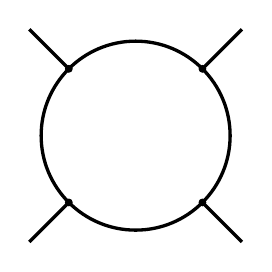
\begin{tikzpicture}[scale=0.6]
\filldraw [color = black, fill=none, very thick] (0,0) circle (2cm);
%\draw [black,very thick] (-2,0) to (2,0);
%\filldraw [black] (2,0) circle (2pt);
%\filldraw [black] (-2,0) circle (2pt);
\filldraw [black] (1.414,1.414) circle (2pt);
\filldraw [black] (-1.414,1.414) circle (2pt);
\filldraw [black] (1.414,-1.414) circle (2pt);
\filldraw [black] (-1.414,-1.414) circle (2pt);
%\draw [black,very thick] (-2,0) to (-3,0);
%\draw [black,very thick] (2,0) to (3,0);
\draw [black,very thick] (1.414,1.414) to (2.25,2.25);
\draw [black,very thick] (-1.414,1.414) to (-2.25,2.25);
\draw [black,very thick] (1.414,-1.414) to (2.25,-2.25);
\draw [black,very thick] (-1.414,-1.414) to (-2.25,-2.25);
\end{tikzpicture}\qquad
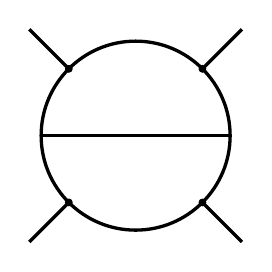
\begin{tikzpicture}[scale=0.6]
\filldraw [color = black, fill=none, very thick] (0,0) circle (2cm);
\draw [black,very thick] (-2,0) to (2,0);
%\filldraw [black] (2,0) circle (2pt);
%\filldraw [black] (-2,0) circle (2pt);
\filldraw [black] (1.414,1.414) circle (2pt);
\filldraw [black] (-1.414,1.414) circle (2pt);
\filldraw [black] (1.414,-1.414) circle (2pt);
\filldraw [black] (-1.414,-1.414) circle (2pt);
%\draw [black,very thick] (-2,0) to (-3,0);
%\draw [black,very thick] (2,0) to (3,0);
\draw [black,very thick] (1.414,1.414) to (2.25,2.25);
\draw [black,very thick] (-1.414,1.414) to (-2.25,2.25);
\draw [black,very thick] (1.414,-1.414) to (2.25,-2.25);
\draw [black,very thick] (-1.414,-1.414) to (-2.25,-2.25);
\end{tikzpicture}
\caption{The box and double-box graphs}\label{fig:ladders}
\end{figure}
\noindent{\bf The massless box graph:}

The graph polynomials are given by
\begin{align}
  \label{e:Boxgraphpolynomials}
  \textbf{U}_{\Box}&=\sum_{i=1}^4 x_i,\cr
  \textbf{F}_{\Box}&=-t x_3x_4-sx_1x_2
\end{align}
with the twisted differential in $D=4-2\epsilon$ in the projective
space $\mathbb P^3$
\begin{equation}\label{e:OmegaBox}
  \Omega_\Box^\epsilon=   {1\over \textbf{F}_{\Box}^2
  }\left(\textbf{U}_{\Box}\over \textbf{F}_{\Box}\right)^\epsilon\,\Omega_0.
\end{equation}
The application of the procedure given in
Section~\ref{sec:deriv-diff-equat} needs only to start at the first
order derivative giving
\begin{equation}
  \mathscr{L}_\Box^\epsilon= (s+t)t {d\over dt}+(s+t+s\epsilon)  
\end{equation}
and the inhomogeneous term
\begin{equation}
  \mathscr{S}_\Box^\epsilon=\frac{(\epsilon +1)\Gamma (-\epsilon -1)^2 }{\Gamma
   (-2 \epsilon )}  \, \left( (-s)^{-1-\epsilon }+(-t)^{-\epsilon -1}\right)
\end{equation}

\noindent{\bf The massless box graph:}

The graph polynomials are given by
\begin{align}
  \label{e:DoubleBoxgraphpolynomials}
  \textbf{U}_{\Box\!\Box}&=(x_1+x_2+x_3)(x_4+x_5+x_6)+(x_1+\cdots+x_6)x_7,\\
\nonumber  \textbf{F}_{\Box\!\Box}&=-t x_3x_5x_7-s\left( (x_1+x_2+x_3) x_4x_6+(x_4+x_5+x_6)x_1x_2+(x_1+x_4)(x_2+x_6)x_7\right)
\end{align}
with the twisted differential in $D=4-2\epsilon$ in the projective
space $\mathbb P^6$
\begin{equation}\label{e:OmegaBox}
  \Omega_{\Box\!\Box}^\epsilon=   {\textbf{U}_{\Box\!\Box}  \over
    \textbf{F}_{\Box\!\Box}^{3}}\left(\textbf{U}_{\Box}\over \textbf{F}_{\Box}\right)^\epsilon\,\Omega_0
\end{equation}



\pvnote{box and 2loop ladder massless}
%%%%%%%%%%%%%%%%%%%%%%%%%%%%%%%%%%%%%%%%%%%%%%%%%%%%%%%%%%%%%%%%%
\section{Minimal order Picard-Fuchs operator and number of master integrals}

The order of the Picard-Fuchs operator and its non-apparent
singularities are determined  the 'motivic' geometry of the Feynman
graph. In the rational case $\epsilon=0$, these are derivable from an
analysis of the Mixed Hodge structure associated to the graph
polynomials~\cite{bek,Brown:2009ta,Doran:2023yzu}.
We compare the results obtained with the generalised Griffiths-Dwork
pole reduction
algorithm and the computation of the Euler characteristic of the
complement of the graph hyper-surface.

The parametric representation of Feynman integrals take different form
but they are all of the type of a generalised Euler integral like the
one in eq.~\eqref{e:FeynPara}. The vector space of the family of these
Euler integrals when varying the powers $(\nu_1,\dots,\nu_n)$ is a
finite dimensional vector space which dimension is given by the Euler
characteristic~\cite{Lee:2013hzt,Bitoun:2017nre,Agostini:2022cgv}
\begin{equation}\label{e:chiGamma}
  \chi_\Gamma:=(-1)^n \chi\left(\underline x\in(\mathbb C^*)^n|
  \textbf{U}_\Gamma(\underline x)\textbf{F}_\Gamma(\underline
  x)\neq0\right).
\end{equation} This number is the so-called number of master
integrals. This provides an upper bound on the minimal order
differential operator acting on the Feynman integral. In the example
studied in this work we have found the following:

\begin{itemize}
\item  For the $n-1$-loop
  sunset integrals, the number of irreducible master integrals for the
  is $2^{n}-n-1$.  The master integrals are given by
  
\begin{itemize}  \item The minimal differential Picard-Fuchs operator for the all
    equal mass case has order  $n-1$
  \item At one-loop $n=2$ we have an operator of order 1, at two-loop
    $n=3$ an operator of order 4 and at three-loop $n=4$ with generic
    mass configuration the Picard-Fuchs operator
as   order 11.  We see that when $\epsilon\neq0$  the order of the
    Picard-Fuchs operator saturates bound given by the number of
    irreducible master.
  \end{itemize}
  \item For the two-loop ice-cream cone the number of irreducible
    master 4 is which is the order of the minimal Picard-Fuchs
    operator for generic kinematics.
  \end{itemize}

For particular choice of the configurations of the internal masses and
external kinematics, it happens that the second Symanzik
$\textbf{F}_\Gamma$ presents some symmetries and the order of the
minimal order Picard-Fuchs operator drops.  This phenomena happens not
only for  the sunset graphs
in~\cite{Bloch:2014qca,Lairez:2022zkj,Bonisch:2021yfw,Bonisch:2020qmm,Pogel:2022vat}
but as well for the other graphs. We have seen in section~\ref{sec:ice-cream} the minimal order Picard-Fuchs
operator for special kinematic configuration of the ice-cream cone
graph is three.
This reduction of order is due to the extra symmetries of the
integrand which gives rise to relations between period integrals.
As explained in~\cite{Lairez:2022zkj} this reduction of order can be
understood by the factorisability of the Picard-Fuchs operator.  The
computation of the Euler characteristic $\chi_\Gamma$ does not detect
these dimension drop. Neither its computation using the critical point
of the
Lee-Pomeransky representation~\cite{Lee:2013hzt}   nor the
Baikov representation~\cite{Frellesvig:2017aai,Frellesvig:2019uqt,Cacciatori:2021nli}.

%----------------------------------------------------------------------
\subsection{interpretation of $\epsilon$ deformations}


For a differential equation
\begin{equation}
  \sum_{r=0}^N c_r(z) {d^rf(z)\over dz^r}=0  
\end{equation}
the roots of $p_N(z)$ are the singularities of the differential
equation. A root of $p_N(z)$ where the solution $f(z)$ is
\emph{regular} is called an apparent singularity.

The non-apparent singularities root of $p_N(z)$ are the roots of the
discriminant of the singular locus of the Feynman integrals~\cite{Doran:2023yzu}.

We have noticed that the $\epsilon$ deformation affects only the
apparent singularities of the differential operator $\mathscr{L}_z^\epsilon$.

The physical reason for this is that in singularities (the threshold
and pseudo-thresholds) of a Feynman integral are independent of the
space-time dimension.  But the local behaviour of the integral near
the thresholds and pseudo-threshold changes with the space-time
dimension.   As fact for instance that has been used with great success
when decomposing amplitudes using the generalized unitarity method~\cite{Bern:2011qt}.

The  $\epsilon$ affects the monodromy of differential equation around
the singular point by changing the indicial equation.





%----------------------------------------------------------------------
\subsection{Two-loop sunset}

For the two-loop sunset the Gauss-Manin connexion is build from the
geometric data of the elliptic curve
$\mathscr{E}_\su:=\{(xy+xz+yz)(m_1^2x_1+m_2^2y+m_3^2z)-t xyz\}$
defined from graph polynomial $\textbf{F}_\su$:
\begin{equation}
  \label{eq:AGM}
  A_{GM}=
  \begin{pmatrix}
    -{1\over 12}{\partial \log\Delta(t)\over \partial t} &{3\over
      2}{\delta\over \Delta}\cr
    -{g_2\over8}{\delta\over\Delta}&{1\over12}{\partial\log\Delta(t)\over\partial t}
  \end{pmatrix}
\end{equation}
For the all equal mass case the Gauss-Manin connexion is
\begin{equation}
  \label{eq:AGM2sunset1mass}
  A_{GM}=\begin{pmatrix}
\frac{-t^{2}+8 t -3}{2 t \left(t -1\right) \left(t -9\right)} & -\frac{3}{2 t \left(t -1\right) \left(t -9\right)} 
\\
 \frac{\left(t -3\right) \left(t^{3}-9 t^{2}+3 t -3\right)}{6 t \left(t -1\right) \left(t -9\right)} & \frac{t^{2}-8 t +3}{2 t \left(t -1\right) \left(t -9\right)} 
\end{pmatrix}
\end{equation}
and the
Picard-Fuchs operator for
in~\eqref{e:PF2sunset1massepsilon} can be obtained from the following
system
\begin{equation}
  {d\over dt}
  \begin{pmatrix}
    I_\su(t)\cr g(t)
  \end{pmatrix} =P(\epsilon,t) A_{GM} \begin{pmatrix}
    I_\su(t)\cr g(t)
  \end{pmatrix},
\end{equation}
with
\begin{equation}
  P(\epsilon,t)=
  \begin{pmatrix}
    1 & 0 
\\
 \frac{\epsilon  \left(2 t^{3} \epsilon -14 \epsilon  \,t^{2}+3 t^{3}-10 \epsilon  t -23 t^{2}+6 \epsilon +29 t -33\right)}{3} & 1+\left(2 t +2\right) \epsilon^{2}+\left(3 t -5\right) \epsilon  
  \end{pmatrix}
\end{equation}

%%%%%%%%%%%%%%%%%%%%%%%%%%%%%%%%%%%%%%%%%%%%%%%%%%%%%%%%%%%%%%%
\section*{Acknowledgements}
We would like to thank Pierre Lairez, Eric Pichon-Pharabod  for discussions.
The work of P.V. has received funding from the ANR grant ``SMAGP''
ANR-20-CE40-0026-01.

%%%%%%%%%%%%%%%%%%%%%%%%%%%%%%%%%%%%%%%%%%%%%%%%%%%%%%%%%%%%%%%
\begin{thebibliography}{99}

\bibitem{Bern:2011qt}
Z.~Bern and Y.~t.~Huang,
``Basics of Generalized Unitarity,''
J. Phys. A \textbf{44} (2011), 454003
doi:10.1088/1751-8113/44/45/454003
[arXiv:1103.1869 [hep-th]].
  
\bibitem{Peraro:2019svx}
T.~Peraro,
``Finiteflow: Multivariate Functional Reconstruction Using Finite Fields and Dataflow Graphs,''
JHEP \textbf{07} (2019), 031
%doi:10.1007/JHEP07(2019)031
[arXiv:1905.08019 [hep-ph]].

  
\bibitem{PutSinger} van der Put, M., and Singer, M. F. Galois Theory of Linear Differential Equations, Vol. 328. Springer: 2003. An electronic version of this book is available at http://www4.ncsu.edu/\~singer/ms\_papers.html.

 \bibitem{vanHoeij} van Hoeij, M. "Factorization of Differential Operators with Rational Functions Coefficients." J. Symb. Comput. Vol. 24. (1997): 537-561.

  
\bibitem{Kawai} Shingo Kawai ``Isomonodromic deformation of Fuchsian projective connections on elliptic curves,'' Nagoya Mathematical Journal, Nagoya Math. J. 171(none), 127-161, (2003)
  
\bibitem{doran-isomo} Charles F. Doran, ``Algebraic and Geometric Isomonodromic Deformations,'' Journal of Differential Geometry 59 (September 2001), no. 1, 33-85 (EN). MR1909248
   
  \bibitem{Sibuya} Yasutaka Sibuya, ``Linear Differential Equations in the Complex Domain: Problems of Analytic Continuation'' (Translations of Mathematical Monographs, 82)

\bibitem{Remiddi:2013joa}
E.~Remiddi and L.~Tancredi,
``Schouten Identities for Feynman Graph Amplitudes; the Master Integrals for the Two-Loop Massive Sunrise Graph,''
Nucl. Phys. B \textbf{880} (2014), 343-377
%doi:10.1016/j.nuclphysb.2014.01.009
[arXiv:1311.3342 [hep-ph]].

  
  \bibitem{Bitoun:2017nre}
T.~Bitoun, C.~Bogner, R.~P.~Klausen and E.~Panzer,
``Feynman Integral Relations from Parametric Annihilators,''
Lett. Math. Phys. \textbf{109} (2019) no.3, 497-564
%doi:10.1007/s11005-018-1114-8
[arXiv:1712.09215 [hep-th]].

\bibitem{Doran:2023yzu}
C.~F.~Doran, A.~Harder, E.~Pichon-Pharabod and P.~Vanhove,
``Motivic Geometry of Two-Loop Feynman Integrals,''
[arXiv:2302.14840 [math.AG]].

\bibitem{Smirnov:2010hn}
A.~V.~Smirnov and A.~V.~Petukhov,
``The Number of Master Integrals is Finite,''
Lett. Math. Phys. \textbf{97} (2011), 37-44
%doi:10.1007/s11005-010-0450-0
[arXiv:1004.4199 [hep-th]].



  \bibitem{Brown:2009ta}
Francis Brown.
\newblock {On the periods of some {F}eynman integrals}.
\newblock 10 2009.
\newblock [arXiv:0910.0114]  

\bibitem{chyzak2022symbolic}
Fr\'{e}d\'{e}ric Chyzak, Alexandre Goyer, and Marc Mezzarobba.
\newblock Symbolic-numeric factorization of differential operators.
\newblock In {\em Proceedings of the 2022 International Symposium on Symbolic
  and Algebraic Computation}, ISSAC '22, page 73-82, New York, NY, USA, 2022.
Association for Computing Machinery.
\newblock [arXiv:2205.08991]

\bibitem{goyer2021sage}
Alexandre Goyer.
\newblock A {S}age package for the symbolic-numeric factorization of linear
  differential operators.
\newblock {\em ACM Communications in Computer Algebra}, 55(2):44--48,
2021.


\bibitem{Griffiths_1969}
P.~A. Griffiths.
\newblock On the periods of certain rational integrals.
\newblock {Ann. of Math.}, {\bf 90} (1969), 460--541.

\bibitem{Dwork_1962}
B.~Dwork.
\newblock On the zeta function of a hypersurface.
\newblock {Inst. Hautes \'Etudes Sci. Publ. Math.} {\bf 12} (1962) 5--68.

\bibitem{Dwork_1964}
B.~Dwork.
\newblock On the zeta function of a hypersurface: {{II}}.
\newblock {Ann. of Math.}, {\bf 80} (1964) 227--299.

\bibitem{lairez2016computing}
Pierre Lairez.
\newblock Computing periods of rational integrals.
\newblock {\em Mathematics of computation}, 85(300):1719--1752, 2016.
\newblock [arXiv:1404.5069]

\bibitem{Eric2023}
Pierre Lairez, Eric Pichon-Pharabod, and Pierre Vanhove.
\newblock {Using effective Picard-Lefschetz theory to compute periods of smooth
  complex projective hypersurfaces,}
\newblock in preparation.



  \bibitem{nakanishi1971graph}
Noboru Nakanishi,
\newblock {\em Graph theory and Feynman integrals}, volume~11.
\newblock Routledge, 1971.


\bibitem{muller2012second}
Stefan M{\"u}ller-Stach, Stefan Weinzierl, and Raphael Zayadeh.
\newblock A second-order differential equation for the two-loop sunrise graph
  with arbitrary masses.
\newblock {\em Communications in Number Theory and Physics}, 6(1):203--222,
2012.
\newblock [arXiv:1112.4360]

\bibitem{muller2014picard}
Stefan M{\"u}ller-Stach, Stefan Weinzierl, and Raphael Zayadeh.
\newblock Picard--{F}uchs equations for {F}eynman integrals.
\newblock {\em Communications in Mathematical Physics},
326(1):237--249, 2014.
\newblock [arXiv:1212.4389]

\bibitem{Weinzierl:2022eaz}
Stefan Weinzierl.
\newblock Quantum field theory.
\newblock In {\em Feynman Integrals: A Comprehensive Treatment for Students and
  Researchers}, pages 101--133. Springer, 2022.
\newblock [arXiv:2201.03593] 


\bibitem{bek}
Spencer Bloch, H{\'e}l{\`e}ne Esnault, and Dirk Kreimer.
\newblock On motives associated to graph polynomials.
\newblock {\em Communications in mathematical physics},
267(1):181--225, 2006.
\newblock [arXiv:math/0510011] 

\bibitem{Bloch:2014qca}
Spencer Bloch, Matt Kerr, and Pierre Vanhove.
\newblock {A Feynman integral via higher normal functions}.
\newblock {\em Compos. Math.}, 151(12):2329--2375, 2015.
\newblock [arXiv:1406.2664] 

\bibitem{Bloch:2016izu}
Spencer Bloch, Matt Kerr, and Pierre Vanhove.
\newblock {Local mirror symmetry and the sunset Feynman integral}.
\newblock {\em Adv. Theor. Math. Phys.}, 21:1373--1453, 2017.
\newblock [arXiv:1601.08181]
  
 \bibitem{PVISSAC} Pierre Vanhove. 2021. ``Differential Equations for Feynman Integrals.'' In Proceedings of the 2021 on International Symposium on Symbolic and Algebraic Computation (ISSAC '21). Association for Computing Machinery, New York, NY, USA, 21-26. https://doi.org/10.1145/3452143.3465512

   \bibitem{Aomoto1} K.~Aomoto, ``Les \'equations aux diff\'erences
     lin\'eaires et les int\'egrales des fonctions multiformes'',
     J. Fac. Sci. Univ. Tokyo, 22(3), 271-297  (1975)
  
  \bibitem{Frellesvig:2017aai}
  H.~Frellesvig and C.~G.~Papadopoulos,
  ``Cuts of Feynman Integrals in Baikov Representation,''
  JHEP {\bf 1704} (2017) 083
%  doi:10.1007/JHEP04(2017)083
  [arXiv:1701.07356 [hep-ph]].

  \bibitem{Aomoto} K.~Aomoto, ``On vanishing of cohomology attached to
    certain many valued meromorphic functions'', J. Math. Soc. Japan
    27(2): 248-255 (1975)

    \bibitem{AomotoBook} K.~Aomoto, K. and M.~Kita, , ``Theory of Hypergeometric Functions,'' Springer Monographs in Mathematics, Springer-Verlag, Tokyo, 2011
    
\bibitem{Cacciatori:2021nli}
S.~L.~Cacciatori, M.~Conti and S.~Trevisan,
``Co-Homology of Differential Forms and Feynman Diagrams,''
Universe \textbf{7} (2021) no.9, 328
doi:10.3390/universe7090328
[arXiv:2107.14721 [hep-th]].
  
\bibitem{Gituliar:2017vzm}
O.~Gituliar and V.~Magerya,
``Fuchsia: a Tool for Reducing Differential Equations for Feynman Master Integrals to Epsilon Form,''
Comput. Phys. Commun. \textbf{219} (2017), 329-338
%doi:10.1016/j.cpc.2017.05.004
[arXiv:1701.04269 [hep-ph]].

\bibitem{Bourjaily:2019hmc}
J.~L.~Bourjaily, A.~J.~McLeod, C.~Vergu, M.~Volk, M.~Von Hippel and M.~Wilhelm,
``Embedding Feynman Integral (Calabi-Yau) Geometries in Weighted Projective Space,''
JHEP \textbf{01} (2020), 078
%doi:10.1007/JHEP01(2020)078
[arXiv:1910.01534 [hep-th]].

\bibitem{Candelas:2021lkc}
P.~Candelas, X.~de la Ossa, P.~Kuusela and J.~McGovern,
``Mirror Symmetry for Five-Parameter Hulek-Verrill Manifolds,''
[arXiv:2111.02440 [hep-th]].

\bibitem{Muller-Stach:2011qkg}
S.~M\"uller-Stach, S.~Weinzierl and R.~Zayadeh,
``A Second-Order Differential Equation for the Two-Loop Sunrise Graph with Arbitrary Masses,''
Commun. Num. Theor. Phys. \textbf{6} (2012), 203-222
%doi:10.4310/CNTP.2012.v6.n1.a5
[arXiv:1112.4360 [hep-ph]].

\bibitem{Remiddi:2016gno}
E.~Remiddi and L.~Tancredi,
``Differential equations and dispersion relations for Feynman amplitudes. The two-loop massive sunrise and the kite integral,''
Nucl. Phys. B \textbf{907} (2016), 400-444
%doi:10.1016/j.nuclphysb.2016.04.013
[arXiv:1602.01481 [hep-ph]].

\bibitem{Chyzak}  Fr\'ed\'eric Chyzak, `` extension of
    Zeilberger's fast algorithm to general holonomic functions'',
Discrete Mathematics, {\bf 217} (1-3) 115-134, 2000.

\bibitem{Bloch:2013tra}
S.~Bloch and P.~Vanhove,
``The elliptic dilogarithm for the sunset graph,''
J. Number Theor. \textbf{148} (2015), 328-364
%doi:10.1016/j.jnt.2014.09.032
[arXiv:1309.5865 [hep-th]].

\bibitem{Bonisch:2020qmm}
K.~B\"onisch, F.~Fischbach, A.~Klemm, C.~Nega and R.~Safari,
``Analytic structure of all loop banana integrals,''
JHEP \textbf{05} (2021), 066
%doi:10.1007/JHEP05(2021)066
[arXiv:2008.10574 [hep-th]].

\bibitem{Chyzak2} Fr\'ed\'eric Chyzak, ``Creative Telescoping for
  Parametrised Integration and Summation'',  Les cours du CIRM,  Vol. 2, no 1 (2011), Course no II, p. 1-37.


\bibitem{Koutchan} C. Koutschan. ``HolonomicFunctions (user's guide).'' Technical Report 10-01, RISC Report Series, Johannes Kepler University, Linz, Austria, 2010. http://www.risc
.jku.at/research/ combinat/software/HolonomicFunctions/.

\bibitem{bostan2013creative} A. Bostan, P. Lairez, and B. Salvy,
  ''Creative telescoping for rational functions using the
  Griffiths--Dwork method.'' In Proceedings of the 38th international
  symposium on symbolic and algebraic computation (pp. 93-100). 
\bibitem{Mizera:2017rqa}
S.~Mizera,
``Scattering Amplitudes from Intersection Theory,''
Phys. Rev. Lett. \textbf{120} (2018) no.14, 141602
%doi:10.1103/PhysRevLett.120.141602
[arXiv:1711.00469 [hep-th]].

\bibitem{Mastrolia:2018uzb}
P.~Mastrolia and S.~Mizera,
``Feynman Integrals and Intersection Theory,''
JHEP \textbf{02} (2019), 139
%doi:10.1007/JHEP02(2019)139
[arXiv:1810.03818 [hep-th]].

\bibitem{Frellesvig:2019uqt}
H.~Frellesvig, F.~Gasparotto, M.~K.~Mandal, P.~Mastrolia, L.~Mattiazzi and S.~Mizera,
``Vector Space of Feynman Integrals and Multivariate Intersection Numbers,''
Phys. Rev. Lett. \textbf{123} (2019) no.20, 201602
%doi:10.1103/PhysRevLett.123.201602
[arXiv:1907.02000 [hep-th]].

\bibitem{Agostini:2022cgv}
D.~Agostini, C.~Fevola, A.~L.~Sattelberger and S.~Telen,
``Vector Spaces of Generalized Euler Integrals,''
[arXiv:2208.08967 [math.AG]].

  
\bibitem{Prausa:2017ltv}
M.~Prausa,
``Epsilon: a Tool to Find a Canonical Basis of Master Integrals,''
Comput. Phys. Commun. \textbf{219} (2017), 361-376
%doi:10.1016/j.cpc.2017.05.026
[arXiv:1701.00725 [hep-ph]].

\bibitem{Aomoto_1982}  K.~Aomoto, ``Configurations and Invariant Gauss-Manin Connections of Integrals I.'' Tokyo Journal of Mathematics 5, 249-287. https://doi.org/10.3836/tjm/1270214894



\bibitem{Lee:2013hzt}
R.~N.~Lee and A.~A.~Pomeransky,
``Critical Points and Number of Master Integrals,''
JHEP \textbf{11} (2013), 165
%doi:10.1007/JHEP11(2013)165
[arXiv:1308.6676 [hep-ph]].
  
\bibitem{Cacciatori:2023tzp}
S.~L.~Cacciatori, H.~Epstein and U.~Moschella,
``Banana Integrals in Configuration Space,''
[arXiv:2304.00624 [hep-th]].
  
\bibitem{Lairez:2022zkj}
P.~Lairez and P.~Vanhove,
``Algorithms for Minimal Picard-Fuchs Operators of Feynman Integrals,''
Lett. Math. Phys. \textbf{113} (2023) no.2, 37
%doi:10.1007/s11005-023-01661-3
[arXiv:2209.10962 [hep-th]].

  
  \bibitem{Vanhove:2014wqa}
P.~Vanhove,
``The Physics and the Mixed Hodge Structure of Feynman Integrals,''
Proc. Symp. Pure Math. \textbf{88} (2014), 161-194
%doi:10.1090/pspum/088/01455
[arXiv:1401.6438 [hep-th]].


\bibitem{Bonisch:2021yfw}
K.~B\"onisch, C.~Duhr, F.~Fischbach, A.~Klemm and C.~Nega,
``Feynman Integrals in Dimensional Regularization and Extensions of Calabi-Yau Motives,''
JHEP \textbf{09} (2022), 156
%doi:10.1007/JHEP09(2022)156
[arXiv:2108.05310 [hep-th]].


\bibitem{Pogel:2022ken}
S.~P\"ogel, X.~Wang and S.~Weinzierl,
``Taming Calabi-Yau Feynman Integrals: the Four-Loop Equal-Mass Banana Integral,''
Phys. Rev. Lett. \textbf{130} (2023) no.10, 101601
%doi:10.1103/PhysRevLett.130.101601
[arXiv:2211.04292 [hep-th]].

\bibitem{Pogel:2022yat}
S.~P\"ogel, X.~Wang and S.~Weinzierl,
``The Three-Loop Equal-Mass Banana Integral in \ensuremath{\varepsilon}-factorised Form with Meromorphic Modular Forms,''
JHEP \textbf{09} (2022), 062
%doi:10.1007/JHEP09(2022)062
[arXiv:2207.12893 [hep-th]].

\bibitem{Pogel:2022vat}
S.~P\"ogel, X.~Wang and S.~Weinzierl,
``Bananas of Equal Mass: Any Loop, Any Order in the Dimensional Regularisation Parameter,''
JHEP \textbf{04} (2023), 117
%doi:10.1007/JHEP04(2023)117
[arXiv:2212.08908 [hep-th]].

\bibitem{Groote:2003ad}
S.~Groote,
``Lectures on Configuration Space Methods for Sunrise Type Diagrams,''
[arXiv:hep-ph/0307290 [hep-ph]].
  
\bibitem{Lebedev} N. N. Lebedev, ``Special Functions and Their
  Applications'', Dover Publications Inc. 

  \bibitem{Forum:2022lpz}
A.~Forum and M.~von Hippel,
``A Symbol and Coaction for Higher-Loop Sunrise Integrals,''
[arXiv:2209.03922 [hep-th]].

\bibitem{sasai} Sasai, T. (1974). ``Monodromy Representations of
  Homology of Certain Elliptic Surfaces.'' Journal of the Mathematical
  Society of Japan, 26(2),
  296-305. https://doi.org/10.2969/jmsj/02620296

  \bibitem{Griffith1} Griffiths, P.A.: The Residue Calculus and Some
    Transcendental Results in Algebraic Geometry, I. Presented at the
    (1966)

    \bibitem{Griffith2} 
    Griffiths, P.A.: ``The Residue Calculus And Some Transcendental
    Results In Algebraic Geometry, II''. Proceedings of the National
    Academy of Sciences. 55, 1392-1395
    (1966). https://doi.org/10.1073/pnas.55.6.1392 
  
  \bibitem{Vanhove:2018mto}
P.~Vanhove,
``Feynman Integrals, Toric Geometry and Mirror Symmetry,''
%doi:10.1007/978-3-030-04480-0\_17
[arXiv:1807.11466 [hep-th]].


\bibitem{Kashiwara:1977nf}
M.~Kashiwara and T.~Kawai, \emph{{Holonomic Systems of Linear Differential
		Equations and Feynman Integrals}},
\href{https://doi.org/10.2977/prims/1195196602}{\emph{Publ. Res. Inst. Math.
		Sci. Kyoto} {\bfseries 12} (1977) 131}.
	
\end{thebibliography}

\end{document}
%%% Local Variables:
%%% mode: latex
%%% TeX-master: t
%%% End:
